\documentclass[conference, a4paper]{IEEEtran}

\usepackage{cite}
\usepackage{amsmath,amssymb,amsfonts}
\usepackage{algorithmic}
\usepackage{graphicx}
\usepackage{textcomp}
\usepackage{xcolor}
\usepackage{hyperref}
\usepackage{listings}
\usepackage{booktabs}
\usepackage{array}
\usepackage{multirow}
\usepackage{enumitem}

\hypersetup{
    colorlinks=true,
    linkcolor=blue!70!black,
    citecolor=green!50!black,
    urlcolor=cyan!70!black
}

\lstdefinestyle{vhdlstyle}{
    basicstyle=\ttfamily\scriptsize,
    breaklines=true,
    captionpos=b,
    frame=single,
    tabsize=2,
    language=VHDL,
    keywordstyle=\color{blue}\bfseries,
    commentstyle=\color{green!60!black}\itshape,
    stringstyle=\color{red!70!black},
    numbers=left,
    numberstyle=\tiny\color{gray},
    numbersep=5pt,
    backgroundcolor=\color{gray!8}
}

\lstdefinestyle{pythonstyle}{
    basicstyle=\ttfamily\scriptsize,
    breaklines=true,
    captionpos=b,
    frame=single,
    tabsize=2,
    language=Python,
    keywordstyle=\color{blue!80!black}\bfseries,
    commentstyle=\color{green!60!black}\itshape,
    stringstyle=\color{orange!80!black},
    numbers=left,
    numberstyle=\tiny\color{gray},
    numbersep=5pt,
    backgroundcolor=\color{gray!8}
}

\lstset{style=vhdlstyle}

\def\BibTeX{{\rm B\kern-.05em{\sc i\kern-.025em b}\kern-.08em
    T\kern-.1667em\lower.7ex\hbox{E}\kern-.125emX}}

\begin{document}

\title{From Silicon to Secret: A Year-Long Dual-Phase Study of Cryptographic Hardware Construction and Physical Side-Channel Exploitation}

\author{\IEEEauthorblockN{Orhun Boydak}
\IEEEauthorblockA{\textit{Cryptography and Hardware Security Research} \\
Ankara, Turkey \\
\href{https://github.com/OrhunBoydak/Hardware-Cryptography-and-SCA}{github.com/OrhunBoydak/Hardware-Cryptography-and-SCA}
}}

\maketitle

\begin{abstract}
Modern computing security is built on the assumption that cryptographic algorithms are mathematically intractable — a belief that holds true in the purely theoretical domain. However, the physical reality of hardware execution introduces a fundamentally different class of vulnerabilities that bypass mathematical hardness entirely. This paper presents a comprehensive, year-long progressive study that deliberately traverses both sides of this boundary: first constructing increasingly sophisticated cryptographic hardware, then systematically dismantling its security through physical side-channel exploitation.

\textbf{Phase 1 (Semester 1 — Construction)} establishes robust hardware cryptographic primitives using VHDL. Starting from the inherent linear weakness of Linear Feedback Shift Registers (LFSRs), a non-linear Shrinking Generator is architected as the first countermeasure. The study then advances to asymmetric public-key systems: a full RSA engine employing Master-Slave Montgomery Multiplication is constructed to eliminate hardware-prohibitive modular division. The Elliptic Curve Cryptography (ECC) mathematical framework is then formally analyzed, with scalar multiplication Point Addition and Point Doubling operations implemented, establishing the groundwork for hardware-efficient ECC accelerators.

\textbf{Phase 2 (Semester 2 — Exploitation)} inverts the lens entirely. A custom RTL-to-Python simulation pipeline parses massive Value Change Dump (VCD) files to achieve perfect, noise-free power modeling, enabling a Correlation Power Analysis (CPA) attack that recovers the full key of the 16-bit RSA system with only 50 simulation traces. The CPA then fails against the 32-bit system due to algorithmic noise — a scientifically quantified finding. Finally, the study bridges simulation to physical reality by instrumenting an Altera DE2-115 FPGA with a precision low-side shunt resistor. A purely algorithmic, knowledge-free peak detection methodology is applied to raw oscilloscope CSV traces, mathematically recovering partial binary key segments through Simple Power Analysis (SPA) — proving the devastating, unconditional effectiveness of timing-based attacks against unprotected hardware.
\end{abstract}

\begin{IEEEkeywords}
Hardware Cryptography, VHDL, FPGA, LFSR, Shrinking Generator, RSA, Montgomery Multiplication, Elliptic Curve Cryptography (ECC), Side-Channel Analysis (SCA), Correlation Power Analysis (CPA), Simple Power Analysis (SPA), Hamming Distance, Pearson Correlation, Altera DE2-115, VCD Parsing.
\end{IEEEkeywords}

% =============================================================================
\section{Introduction and Research Motivation}
% =============================================================================

The security of modern digital infrastructure rests on two intertwined pillars: the mathematical hardness of cryptographic primitives and the physical integrity of the hardware executing them. Classical cryptanalysis attacks the first pillar; Side-Channel Analysis (SCA) attacks the second. The core insight behind SCA — that the \textit{physical behavior} of executing a computation leaks information about the secret being computed — was first formally demonstrated by Paul Kocher et al. in 1999 \cite{b3} and has since grown into one of the most actively researched and industrially relevant fields in embedded security.

\subsection{Motivation: The Gap Between Algorithm and Implementation}
A textbook RSA implementation is computationally secure under the assumption that factoring an $N$-bit modulus is infeasible. This is mathematically true. Yet every time the hardware computes a Montgomery multiplication, the switching activity of its flip-flops — measured in milliamps across a 0.5 $\Omega$ shunt resistor — broadcasts the Hamming weight of the intermediate result directly to any oscilloscope probe. The algorithm is unbroken; the device is not.

This gap between \textit{algorithmic security} and \textit{implementation security} is the central thesis of this year-long research program. Understanding both sides rigorously requires the researcher to wear two distinct hats: the hardware architect who constructs the system, and the attacker who understands precisely which physical phenomena to measure and how to extract secrets from them.

\subsection{Research Objectives}
This study is structured around four progressive research objectives:
\begin{enumerate}[leftmargin=*, label=\textbf{O\arabic*.}]
    \item \textbf{Stream Cipher Hardening:} Design and verify a non-linear VHDL stream cipher that provably resists the Berlekamp-Massey algorithm.
    \item \textbf{Asymmetric Hardware Engine:} Implement a complete RSA modular exponentiation engine in VHDL using Montgomery arithmetic, eliminating hardware-prohibitive integer division.
    \item \textbf{Simulated CPA:} Develop a Python pipeline to parse GHDL simulation outputs and execute a statistically rigorous Correlation Power Analysis attack, quantifying the effect of datapath width on attack success.
    \item \textbf{Physical SPA on FPGA:} Instrument an Altera DE2-115 FPGA for real current measurement, capture power traces with an oscilloscope, and execute a blind key-extraction algorithm without any prior knowledge of the secret key.
\end{enumerate}

\subsection{Paper Organization}
Section~\ref{sec:theory} establishes all mathematical and hardware-security foundations. Sections~\ref{sec:lfsr} through \ref{sec:ecc} detail the Phase 1 hardware construction. Sections~\ref{sec:cpa} and \ref{sec:spa} detail the Phase 2 attack experiments. Section~\ref{sec:conclusion} synthesizes conclusions and countermeasure recommendations.

% =============================================================================
\section{Theoretical Background and Mathematical Foundations}
\label{sec:theory}
% =============================================================================

Before addressing implementations and attacks, this section formally establishes the mathematical infrastructure upon which all subsequent work is built.

\subsection{Linear Feedback Shift Registers: Structure and Weakness}

A Linear Feedback Shift Register (LFSR) is a sequential circuit consisting of $N$ delay elements (D-type flip-flops) connected in a shift register topology, with the input driven by a \textit{linear} combination of selected state bits. The term ``linear'' here has a precise algebraic meaning: the feedback function is computed exclusively using XOR gates, which corresponds to addition over the Galois Field $GF(2)$.

\subsubsection*{Mathematical Model}
Let $s_i \in GF(2)$ denote the state bit at position $i$ at time $t$. For an $N$-bit LFSR with feedback taps at positions $\{c_1, c_2, \ldots, c_k\}$, the next output bit $s_{N+t}$ is:
\begin{equation}
    s_{N+t} = c_1 s_{N+t-1} \oplus c_2 s_{N+t-2} \oplus \cdots \oplus c_k s_{N+t-k}
\end{equation}
This recurrence has a characteristic polynomial $f(x) = 1 + c_1 x + c_2 x^2 + \cdots + c_k x^k$ over $GF(2)$. The LFSR achieves its maximum possible period of $2^N - 1$ states (the all-zero state is forbidden, as it is an absorbing state under XOR feedback) if and only if $f(x)$ is a \textbf{Primitive Polynomial} over $GF(2)$.

\subsubsection*{The Fatal Linearity Flaw}
Despite their extraordinary efficiency in hardware (only flip-flops and XOR gates are required), LFSRs are cryptographically broken as standalone stream ciphers. The Berlekamp-Massey algorithm \cite{b5} can reconstruct the feedback polynomial — and therefore the entire future output sequence — given only $2N$ consecutive output bits. An attacker intercepting $128$ bits of an $N=64$ LFSR output can solve a system of $64$ linear equations over $GF(2)$ to uniquely determine all tap positions and the current internal state. This is the fundamental design deficiency that the Shrinking Generator resolves.

\subsection{RSA Public-Key Cryptography and Modular Arithmetic}

RSA (Rivest-Shamir-Adleman, 1977) \cite{b6} is an asymmetric cryptosystem whose security relies on the \textbf{Integer Factorization Problem}: given a composite integer $N = p \cdot q$ where $p$ and $q$ are large primes, factoring $N$ back into its components is computationally infeasible for sufficiently large $N$.

\subsubsection*{Key Generation}
Select two distinct, large primes $p$ and $q$. Compute the modulus $N = p \cdot q$. Compute Euler's totient:
\begin{equation}
    \phi(N) = (p-1)(q-1)
\end{equation}
Choose a public exponent $e$ such that $1 < e < \phi(N)$ and $\gcd(e, \phi(N)) = 1$. Compute the private exponent $d$ as the modular multiplicative inverse of $e$:
\begin{equation}
    d \equiv e^{-1} \pmod{\phi(N)}, \quad \text{i.e.,} \quad e \cdot d \equiv 1 \pmod{\phi(N)}
\end{equation}
The public key is $(e, N)$; the private key is $(d, N)$.

\subsubsection*{Encryption and Decryption}
Given plaintext $M$ (where $0 \leq M < N$), ciphertext $C$ and recovered message $M'$ are:
\begin{equation}
    C = M^e \pmod{N}, \qquad M' = C^d \pmod{N}
\end{equation}
Correctness follows directly from Euler's theorem: $M^{\phi(N)} \equiv 1 \pmod{N}$, so $M^{ed} = M^{1 + k\phi(N)} \equiv M \pmod{N}$.

\subsubsection*{The Hardware Challenge: Modular Reduction Without Division}
For production RSA with $N$ of 2048 bits, computing $M^e \pmod{N}$ via naive methods requires division of numbers with thousands of bits. Hardware integer dividers are prohibitively expensive in area and latency. This directly motivates the Montgomery Multiplication algorithm.

\subsubsection*{Square-and-Multiply Algorithm}
Modular exponentiation is computed iteratively via the Left-to-Right Binary Method (Algorithm~\ref{alg:sqm}), which scans exponent bits from MSB to LSB, performing at most $2\log_2(d)$ modular multiplications.

\begin{algorithmic}
\STATE \textbf{Input:} Base $M$, exponent $d = (d_{n-1}, d_{n-2}, \ldots, d_0)_2$, modulus $N$
\STATE \textbf{Output:} $M^d \pmod{N}$
\STATE $R \leftarrow 1$
\FOR{$i = n-1$ \textbf{downto} $0$}
    \STATE $R \leftarrow R^2 \pmod{N}$ \hfill \texttt{(SQUARE)}
    \IF{$d_i = 1$}
        \STATE $R \leftarrow R \cdot M \pmod{N}$ \hfill \texttt{(MULTIPLY)}
    \ENDIF
\ENDFOR
\RETURN $R$
\end{algorithmic}
\vspace{2pt}
\textit{Algorithm 1: Square-and-Multiply for Modular Exponentiation.}
\vspace{4pt}

This branching behavior is the root cause of SPA vulnerability: a key bit '1' triggers two operations while a '0' triggers one, producing a measurable difference in execution time and power profile.

\subsubsection*{Montgomery Multiplication}
Peter Montgomery's 1985 algorithm \cite{b2} eliminates division by performing all modular arithmetic in the \textbf{Montgomery domain}. Given a modulus $N$ and a transformation parameter $R = 2^k$ where $k \geq \log_2 N$ and $\gcd(R, N) = 1$, the Montgomery form of an integer $a$ is $\tilde{a} = aR \pmod{N}$.

The \textbf{Montgomery Product} $\text{MonPro}(\tilde{a}, \tilde{b})$ computes $\tilde{a} \cdot \tilde{b} \cdot R^{-1} \pmod{N}$ using only addition and right-shifts — hardware-trivial operations:
\begin{equation}
    \text{MonPro}(\tilde{a}, \tilde{b}) = \tilde{a} \cdot \tilde{b} \cdot R^{-1} \pmod{N}
\end{equation}
The iterative hardware algorithm processes one bit of $\tilde{a}$ at a time, conditionally adding $\tilde{b}$ and performing a modular adjustment via addition (never division). Conversion back to the standard domain at the end requires one final multiplication by $1 \pmod{N}$ (the domain-exit operation).

\subsection{Elliptic Curve Cryptography (ECC)}

Elliptic Curve Cryptography, independently proposed by Miller \cite{b7} and Koblitz \cite{b4} in 1985--1987, provides cryptographic security equivalent to RSA but with dramatically smaller key sizes. The security of ECC relies on the \textbf{Elliptic Curve Discrete Logarithm Problem (ECDLP)}: given points $P$ and $Q = kP$ on an elliptic curve, it is computationally infeasible to recover the scalar $k$.

\subsubsection*{Curve Definition}
A short Weierstrass curve over a prime field $GF(p)$ is defined by:
\begin{equation}
    E: \quad y^2 \equiv x^3 + ax + b \pmod{p}
\end{equation}
subject to the non-singularity condition $4a^3 + 27b^2 \not\equiv 0 \pmod{p}$, which ensures no cusps or self-intersections exist. Points satisfying this equation, together with the ``point at infinity'' $\mathcal{O}$, form an abelian group under the geometric addition law.

\subsubsection*{Group Operations}
Two fundamental geometric operations define ECC arithmetic:

\textbf{Point Addition ($P + Q = R$):} For distinct points $P = (x_1, y_1)$ and $Q = (x_2, y_2)$:
\begin{align}
    \lambda &= \frac{y_2 - y_1}{x_2 - x_1} \pmod{p} \\
    x_3 &= \lambda^2 - x_1 - x_2 \pmod{p} \\
    y_3 &= \lambda(x_1 - x_3) - y_1 \pmod{p}
\end{align}

\textbf{Point Doubling ($P + P = 2P$):} For a single point $P = (x_1, y_1)$:
\begin{align}
    \lambda &= \frac{3x_1^2 + a}{2y_1} \pmod{p} \\
    x_3 &= \lambda^2 - 2x_1 \pmod{p} \\
    y_3 &= \lambda(x_1 - x_3) - y_1 \pmod{p}
\end{align}

\textbf{Scalar Multiplication ($Q = kP$):} Analogous to Square-and-Multiply for RSA, the \textbf{Double-and-Add} algorithm iteratively applies the above two operations, scanning bits of $k$ to compute $Q$. This is the core operation for both key generation and encryption in ECC protocols (ECDH, ECDSA).

\subsubsection*{ECC vs. RSA: Hardware Efficiency Comparison}
Table~\ref{tab:ecc_vs_rsa} quantifies the key size and operational equivalence between RSA and NIST-standardized ECC curves, directly motivating ECC adoption in resource-constrained hardware.

\begin{table}[htbp]
\centering
\caption{Security Level Comparison: RSA vs. ECC}
\label{tab:ecc_vs_rsa}
\begin{tabular}{>{\centering\arraybackslash}p{1.6cm}|>{\centering\arraybackslash}p{1.8cm}|>{\centering\arraybackslash}p{1.8cm}|>{\centering\arraybackslash}p{1.5cm}}
\toprule
\textbf{Security} & \textbf{RSA Key} & \textbf{ECC Key} & \textbf{Size} \\
\textbf{(bits)} & \textbf{(bits)} & \textbf{(bits)} & \textbf{Ratio} \\
\midrule
80  & 1024  & 160  & 6.4$\times$ \\
112 & 2048  & 224  & 9.1$\times$ \\
128 & 3072  & 256  & 12$\times$  \\
192 & 7680  & 384  & 20$\times$  \\
256 & 15360 & 521  & 29$\times$  \\
\bottomrule
\end{tabular}
\end{table}

\subsection{Side-Channel Analysis: Physical Leakage Model}

\subsubsection*{CMOS Power Model}
Standard CMOS logic gates consume power in three regimes: static leakage (negligible), short-circuit transient current (small), and \textbf{dynamic switching power}:
\begin{equation}
    P_\text{dynamic} = \alpha \cdot C_L \cdot V_{DD}^2 \cdot f_{clk}
\end{equation}
where $\alpha$ is the \textit{switching activity factor} — the fraction of transitions occurring per clock cycle. Since $C_L$, $V_{DD}$, and $f_{clk}$ are fixed for a given device, instantaneous power is directly proportional to $\alpha$, which is itself a function of the specific data values being processed.

\subsubsection*{Hamming Distance Leakage Model}
When a register transitions from value $V_\text{old}$ to $V_\text{new}$, the number of bit transitions is the \textbf{Hamming Distance}:
\begin{equation}
    HD(V_\text{old}, V_\text{new}) = HW(V_\text{old} \oplus V_\text{new}) = \sum_{i=0}^{N-1} \left[(V_\text{old})_i \oplus (V_\text{new})_i\right]
\end{equation}
where $HW(\cdot)$ denotes the Hamming Weight (population count). This model is the industry-standard approximation for the instantaneous power consumed by a digital register during a clock edge.

\subsubsection*{Simple Power Analysis (SPA)}
SPA exploits \textit{macroscopic} control-flow differences visible in a single or few power traces. For the Square-and-Multiply algorithm, a key bit $d_i = 0$ triggers only a SQUARE state (duration $\Delta T_S$), while $d_i = 1$ triggers SQUARE followed by MULTIPLY (duration $\Delta T_S + \Delta T_M$). An attacker measuring these durations directly reads the secret key — no statistics required. SPA is the most immediate threat to naive hardware implementations.

\subsubsection*{Correlation Power Analysis (CPA)}
CPA \cite{b3} is a statistical attack that recovers keys even when individual leakages are buried in noise. The attacker collects $N$ power traces $\{T_i(t)\}$ for $N$ known inputs, then for each sub-key hypothesis $k_j$, computes a theoretical power matrix $H_{i,j} = HD(\text{model}(k_j, \text{input}_i))$. The Pearson correlation between the hypothesis column $H_j$ and each sample point $T(t)$ is:
\begin{equation}
    r(H_j, T(t)) = \frac{\sum_{i=1}^{N}(H_{i,j} - \bar{H}_j)(T_i(t) - \bar{T}(t))}{\sqrt{\sum_i(H_{i,j}-\bar{H}_j)^2} \cdot \sqrt{\sum_i(T_i(t)-\bar{T}(t))^2}}
\end{equation}
The correct key hypothesis produces $|r| \approx 1$ at the clock cycle where the modeled register updates, while incorrect hypotheses remain near $|r| \approx 0$.

% =============================================================================
\section{Phase 1 — Semester 1: Stream Cipher Hardening}
\label{sec:lfsr}
% =============================================================================

\subsection{Background and Design Rationale}

The first laboratory objective was to implement a hardware stream cipher that generates cryptographically usable keystreams. The natural starting point — a standalone LFSR — provides maximal-length sequences and exceptional hardware efficiency but fails cryptographically due to its linearity.

The question was: \textit{what is the minimum architectural addition needed to destroy LFSR linearity while preserving hardware simplicity?}

The answer, proven mathematically by Meier and Staffelbach in 1993 \cite{b1}, is the \textbf{Shrinking Generator}: a two-LFSR structure where one LFSR acts as a non-linear decimator (selector) of the other's output.

\subsection{The LFSR Module: Generic VHDL Architecture}

The base LFSR module was designed as a fully generic VHDL entity, parameterized by bit width and tap mask, enabling instantiation of any Fibonacci-form LFSR without code duplication:

\begin{lstlisting}[style=vhdlstyle, caption={Generic LFSR Entity — Parameterized Primitive Polynomial Engine}, label={lst:lfsr}]
entity lfsr is
    Generic (
        WIDTH    : integer := 64;
        TAP_MASK : std_logic_vector
    );
    Port (
        clk     : in  STD_LOGIC;
        rst     : in  STD_LOGIC;
        out_bit : out STD_LOGIC  -- MSB output
    );
end lfsr;

architecture Behavioral of lfsr is
    signal r_reg    : std_logic_vector(WIDTH-1 downto 0)
                    := (0 => '1', others => '0');
    signal feedback : std_logic;
begin
    -- XOR all tapped bits to generate feedback
    process(r_reg)
        variable v_xor : std_logic;
    begin
        v_xor := '0';
        for i in 0 to WIDTH-1 loop
            if TAP_MASK(i) = '1' then
                v_xor := v_xor xor r_reg(i);
            end if;
        end loop;
        feedback <= v_xor;
    end process;

    process(clk, rst)
    begin
        if rst = '1' then
            r_reg <= (0 => '1', others => '0');
        elsif rising_edge(clk) then
            r_reg <= r_reg(WIDTH-2 downto 0) & feedback;
        end if;
    end process;

    out_bit <= r_reg(WIDTH-1);
end Behavioral;
\end{lstlisting}

\subsubsection*{Design Decisions}
\begin{itemize}
    \item \textbf{Seed initialization:} The reset state is hardcoded to $(1, 0, 0, \ldots, 0)$ to avoid the all-zero absorbing state, a common implementation error.
    \item \textbf{Fibonacci vs. Galois form:} Fibonacci form was selected for clarity and ease of tap verification, at the cost of a slightly longer feedback combinational path.
    \item \textbf{Generic TAP\_MASK:} Allows compile-time selection of any primitive polynomial by setting the corresponding bit positions to '1'.
\end{itemize}

\subsection{Primitive Polynomials and Period Analysis}

For the Shrinking Generator, two LFSRs of \textit{coprime} lengths were selected to maximize the combined output period. This is a critical cryptographic requirement: if $\gcd(N_A, N_B) > 1$, the combined period is $(2^{N_A}-1)(2^{N_B}-1) / \gcd(\ldots)$, which is shorter than optimal.

\begin{itemize}
    \item \textbf{LFSR A (64-bit, Selector):} Polynomial $x^{64} + x^4 + x^3 + x + 1$. Period = $2^{64} - 1 \approx 1.8 \times 10^{19}$.
    \item \textbf{LFSR B (63-bit, Data):} Polynomial $x^{63} + x + 1$. Period = $2^{63} - 1 \approx 9.2 \times 10^{18}$.
    \item \textbf{Combined period:} Since $\gcd(64, 63) = 1$, the Shrinking Generator's output period is approximately $(2^{64}-1)(2^{63}-1)/2 \approx 2^{126}$ — far beyond any brute-force attack.
\end{itemize}

\subsection{Shrinking Generator: Non-Linearity Through Decimation}

The Shrinking Generator connects LFSR A as a real-time controller over LFSR B's output. The control logic is remarkably simple:

\begin{lstlisting}[style=vhdlstyle, caption={Shrinking Generator — Asynchronous Master-Slave LFSR}, label={lst:shrink}]
process(clk, rst)
begin
    if rst = '1' then
        stream_out <= '0';
        valid_out  <= '0';
    elsif rising_edge(clk) then
        if bit_A_select = '1' then
            stream_out <= bit_B_data; -- Pass B's bit
            valid_out  <= '1';        -- Mark as valid
        else
            valid_out  <= '0';        -- Shrink (discard B's bit)
        end if;
    end if;
end process;
\end{lstlisting}

\subsubsection*{Why This Destroys Linearity}
The output is an \textit{irregular decimation} of LFSR B's sequence controlled by LFSR A. Although both component sequences are linear, the irregular sampling introduced by A renders the output non-linear. Specifically:
\begin{itemize}
    \item The time index at which LFSR B's output is sampled is unpredictable (it depends on the secret initialization of A).
    \item The Berlekamp-Massey algorithm requires equally-spaced samples; the irregular timing of \texttt{valid\_out} makes the output sequence unattackable by linear algebra.
    \item The minimum linear complexity of the Shrinking Generator output is approximately $2^{n_A-1} \cdot n_B$ — astronomically larger than the $2N$ required to break a raw LFSR.
\end{itemize}

\begin{figure}[htbp]
\centerline{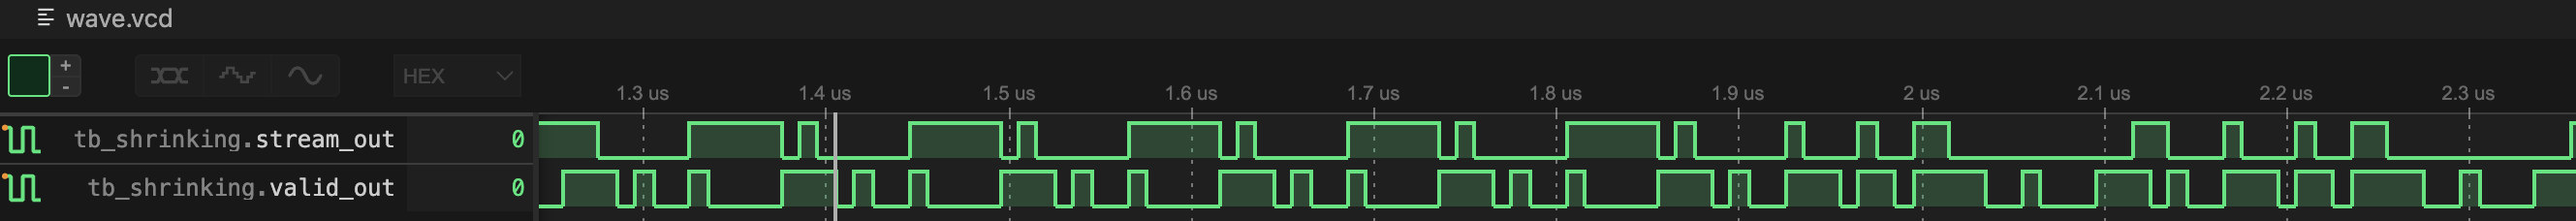
\includegraphics[width=\columnwidth]{images/LFSR1.png}}
\caption{GHDL simulation waveform of the Shrinking Generator. The \texttt{valid\_out} signal asynchronously pulses when LFSR A outputs '1', decimating LFSR B's stream. The irregular timing intervals between valid pulses visually confirm the destruction of temporal linearity.}
\label{fig:lfsr1}
\end{figure}

As shown in Fig.~\ref{fig:lfsr1}, the simulation confirms that the output appears in irregular bursts, completely eliminating the periodicity that would allow linear prediction.

% =============================================================================
\section{Phase 1 — Semester 1: RSA Hardware Engine}
\label{sec:rsa}
% =============================================================================

\subsection{Background and Architectural Challenge}

Having established stream cipher security, the research progressed to asymmetric cryptography — specifically, implementing RSA hardware that is both functionally correct and physically realizable. The central engineering challenge is the cost of modular arithmetic: computing $M^d \pmod{N}$ for multi-kilobit operands requires thousands of modular multiplications, each involving large-integer division. A naive hardware divider for 2048-bit operands would require enormous silicon area and dominate the critical path.

The architectural solution adopted is \textbf{Montgomery's algorithm}: by transforming operands into the Montgomery domain, all modular reductions become simple bit-shifts and additions — operations that map directly to primitive hardware elements.

\subsection{The Montgomery Multiplier Slave FSM}

The Montgomery product module (\texttt{mon\_pro}) implements the bit-serial Montgomery algorithm as a Slave Finite State Machine with three states: \texttt{IDLE}, \texttt{COMPUTE}, and \texttt{DONE}. During the \texttt{COMPUTE} phase, it iterates through each bit of the multiplier, conditionally accumulates the multiplicand, and performs the Montgomery reduction:

\begin{lstlisting}[style=vhdlstyle, caption={Montgomery Multiplier Core Loop — Bit-Serial Reduction}, label={lst:montgomery}]
-- Bit-serial Montgomery product core (simplified)
process(clk)
    variable t : unsigned(WIDTH downto 0) := (others => '0');
begin
    if rising_edge(clk) then
        if a_bit = '1' then
            t := t + unsigned(b);   -- Conditional add
        end if;
        if t(0) = '1' then
            t := t + unsigned(n);   -- Modular adjustment
        end if;
        t := '0' & t(WIDTH downto 1); -- Right-shift = / 2
    end if;
end process;
\end{lstlisting}

The right-shift by 1 at each iteration implements the $R^{-1}$ factor of Montgomery multiplication. Since $R = 2^{WIDTH}$, shifting right by 1 bit for each of the $WIDTH$ iterations cumulatively divides by $R$, completing the Montgomery product without ever invoking integer division.

\begin{figure}[htbp]
\centerline{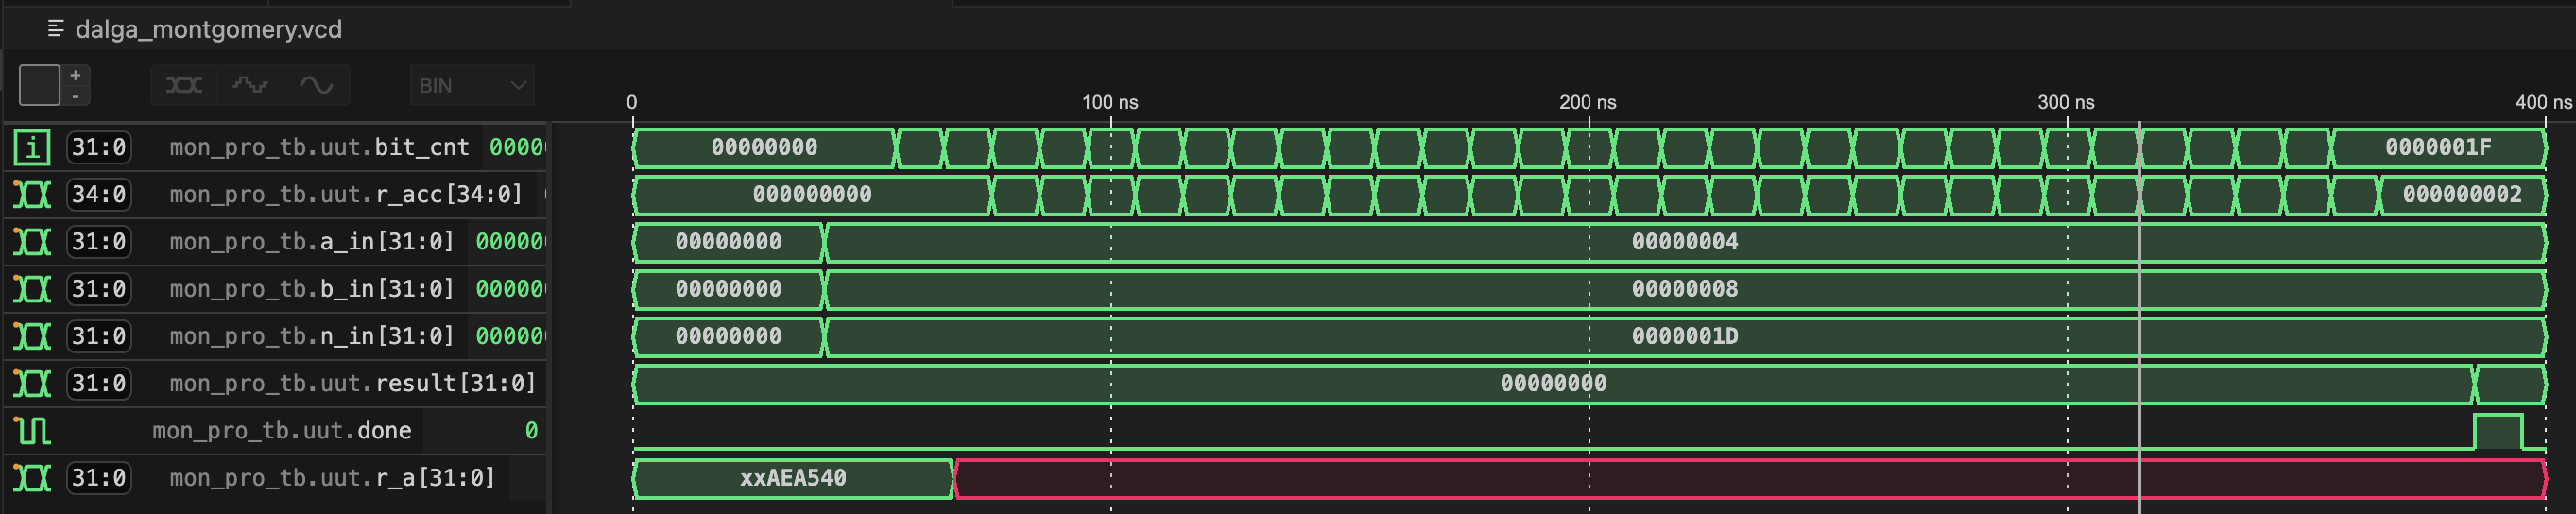
\includegraphics[width=\columnwidth]{images/RSA_montgomery.png}}
\caption{Internal waveforms of the Montgomery Multiplier completing a full multiplication cycle. Each row of clock cycles corresponds to processing one bit of the multiplicand. The conditional additions and right-shifts are visible in the data bus transitions. The \texttt{done} flag rises when all $N$ bits have been processed.}
\label{fig:rsa_montgomery}
\end{figure}

\subsection{Master FSM: Square-and-Multiply Orchestrator}

The Master FSM (\texttt{mod\_exp}) controls the Square-and-Multiply algorithm and orchestrates the Montgomery Slave. It operates in an 8-state machine with the following control flow:

\begin{enumerate}
    \item \textbf{INIT:} Load operands; compute initial Montgomery conversions.
    \item \textbf{SCAN:} Read the current MSB of the private exponent.
    \item \textbf{SQUARE:} Assert the Montgomery multiplier for a squaring operation ($R = R^2 \pmod{N}$). Wait for \texttt{done}.
    \item \textbf{CHECK:} If the scanned key bit is '1', proceed to MULTIPLY.
    \item \textbf{MULTIPLY:} Assert the Montgomery multiplier for $R = R \times M \pmod{N}$. Wait for \texttt{done}.
    \item \textbf{SHIFT:} Advance to the next exponent bit.
    \item \textbf{FINALIZE:} Multiply by 1 to exit the Montgomery domain.
    \item \textbf{DONE:} Output the result and assert \texttt{done\_flag}.
\end{enumerate}

\begin{figure}[htbp]
\centerline{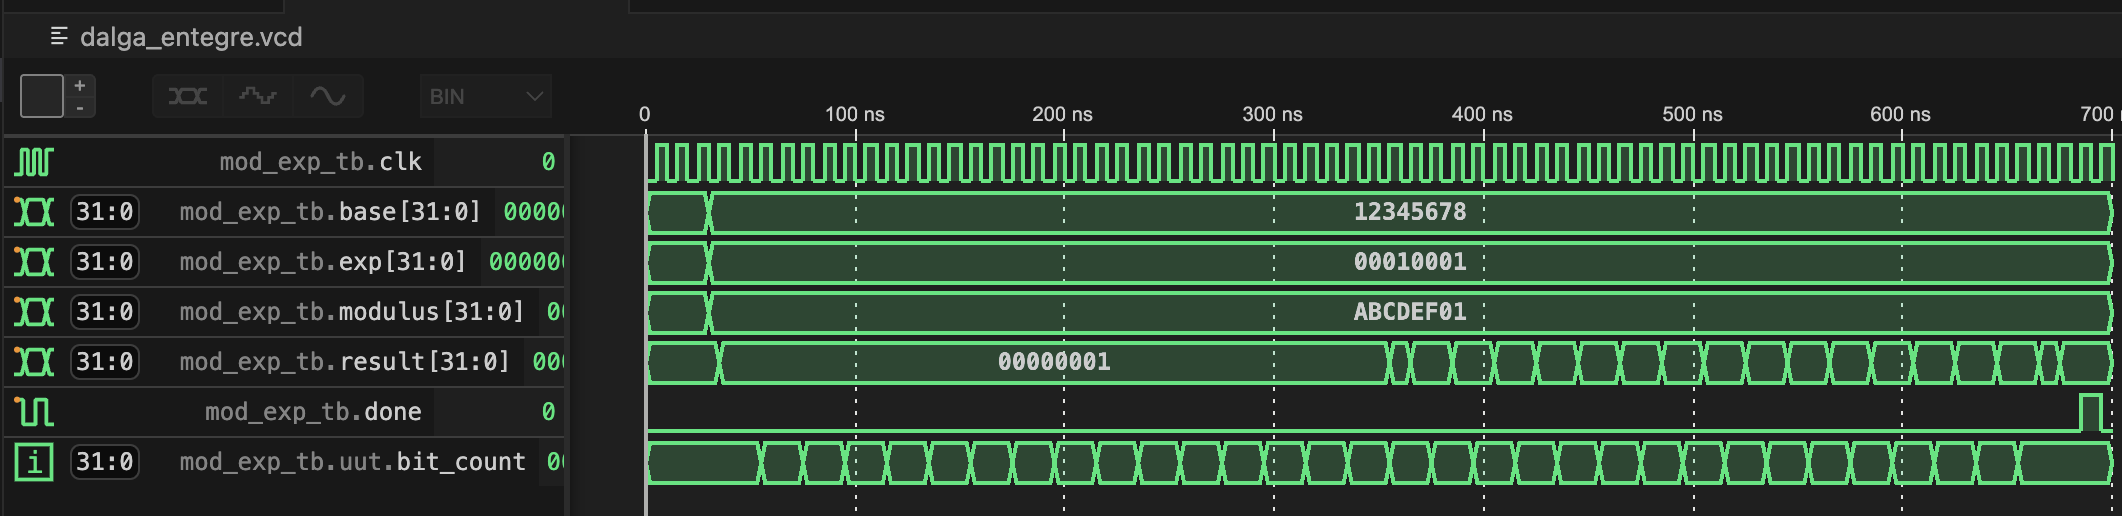
\includegraphics[width=\columnwidth]{images/RSA_engine.png}}
\caption{Master FSM state transitions for the Square-and-Multiply engine. The tight \texttt{SQUARE $\rightarrow$ CHECK $\rightarrow$ MULTIPLY} loop is clearly visible, along with the \texttt{done} handshake between Master and Slave (Montgomery) sub-module.}
\label{fig:rsa_engine}
\end{figure}

\subsection{16-bit and 32-bit Verification}

Both a 16-bit and a 32-bit variant were implemented and verified in simulation. The 16-bit variant uses small, hand-verifiable prime pairs ($p=3, q=11, N=33, \phi=20, e=3, d=7$), allowing manual cross-checking. The 32-bit extends the architecture to larger operands, increasing the Montgomery loop count and correspondingly increasing the simulation trace length.

\begin{figure}[htbp]
\centerline{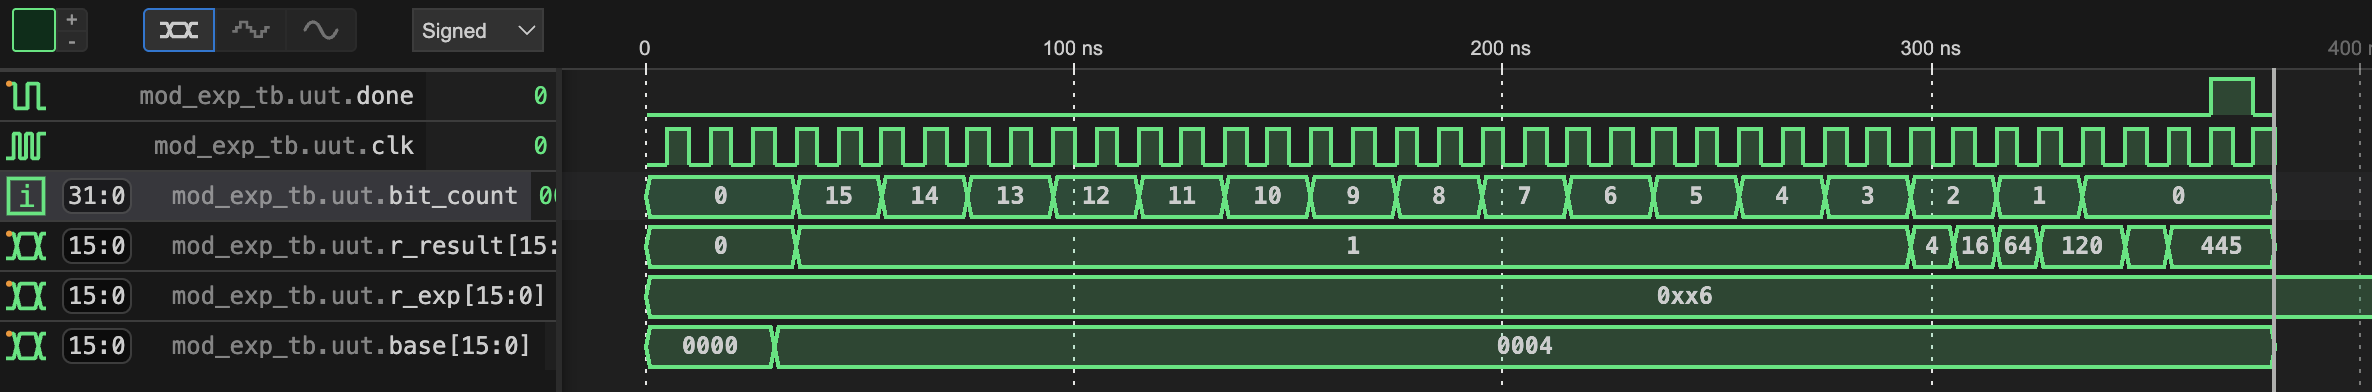
\includegraphics[width=\columnwidth]{images/RSA_16bit.png}}
\caption{16-bit RSA simulation waveform. The engine correctly computes $C = M^e \pmod{N}$ and $M' = C^d \pmod{N}$, with $M' = M$ confirming mathematical correctness.}
\label{fig:rsa_16bit}
\end{figure}

\begin{figure}[htbp]
\centerline{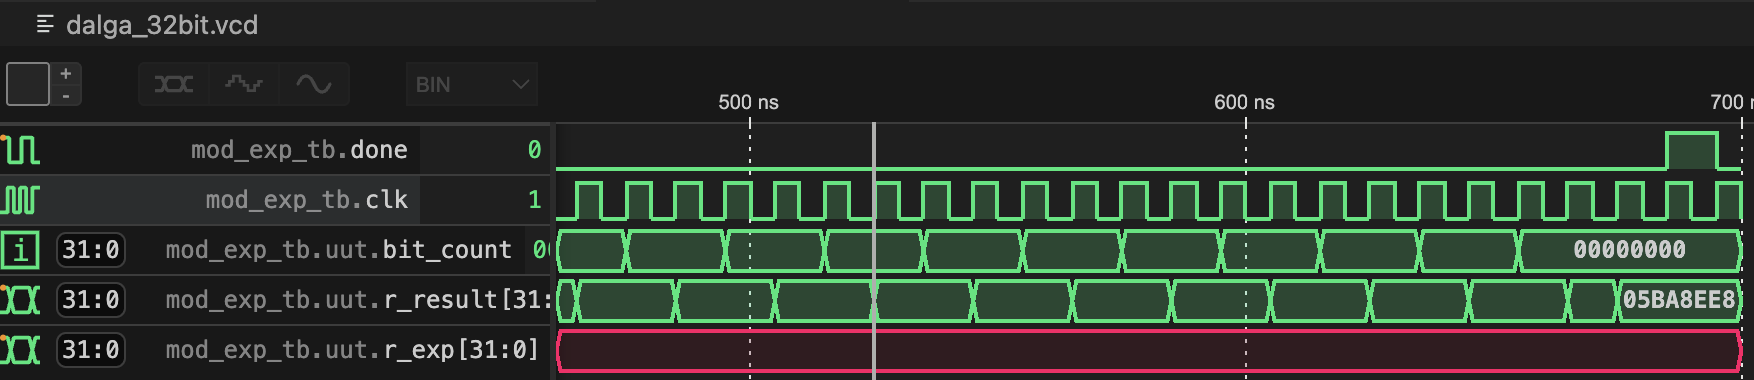
\includegraphics[width=\columnwidth]{images/RSA_32bit.png}}
\caption{32-bit RSA simulation: wider datapath requires more Montgomery iterations per key bit, producing a longer but structurally identical execution trace.}
\label{fig:rsa_32bit}
\end{figure}

% =============================================================================
\section{Phase 1 — Semester 1: ECC Mathematical Framework}
\label{sec:ecc}
% =============================================================================

\subsection{Motivation: RSA Limitations in Constrained Hardware}

As demonstrated in Table~\ref{tab:ecc_vs_rsa}, RSA requires modulus sizes 12--29$\times$ larger than ECC to achieve equivalent security. For an embedded or IoT hardware context — where silicon area, power budget, and clock frequency are severely constrained — RSA's bloated key material is a fundamental engineering liability. ECC was therefore studied as the natural next evolution in cryptographic hardware architecture.

\subsection{The Double-and-Add Algorithm as a Hardware Control Flow}

ECC scalar multiplication $Q = kP$ is computed by the Double-and-Add algorithm: scan bits of $k$ from MSB to LSB. For each bit, always double the accumulator. If the bit is '1', additionally add $P$. This is the exact structural twin of RSA's Square-and-Multiply — an insight with profound SCA implications: \textit{ECC is also vulnerable to the same SPA timing attack if implemented without countermeasures}.

\begin{figure}[htbp]
\centerline{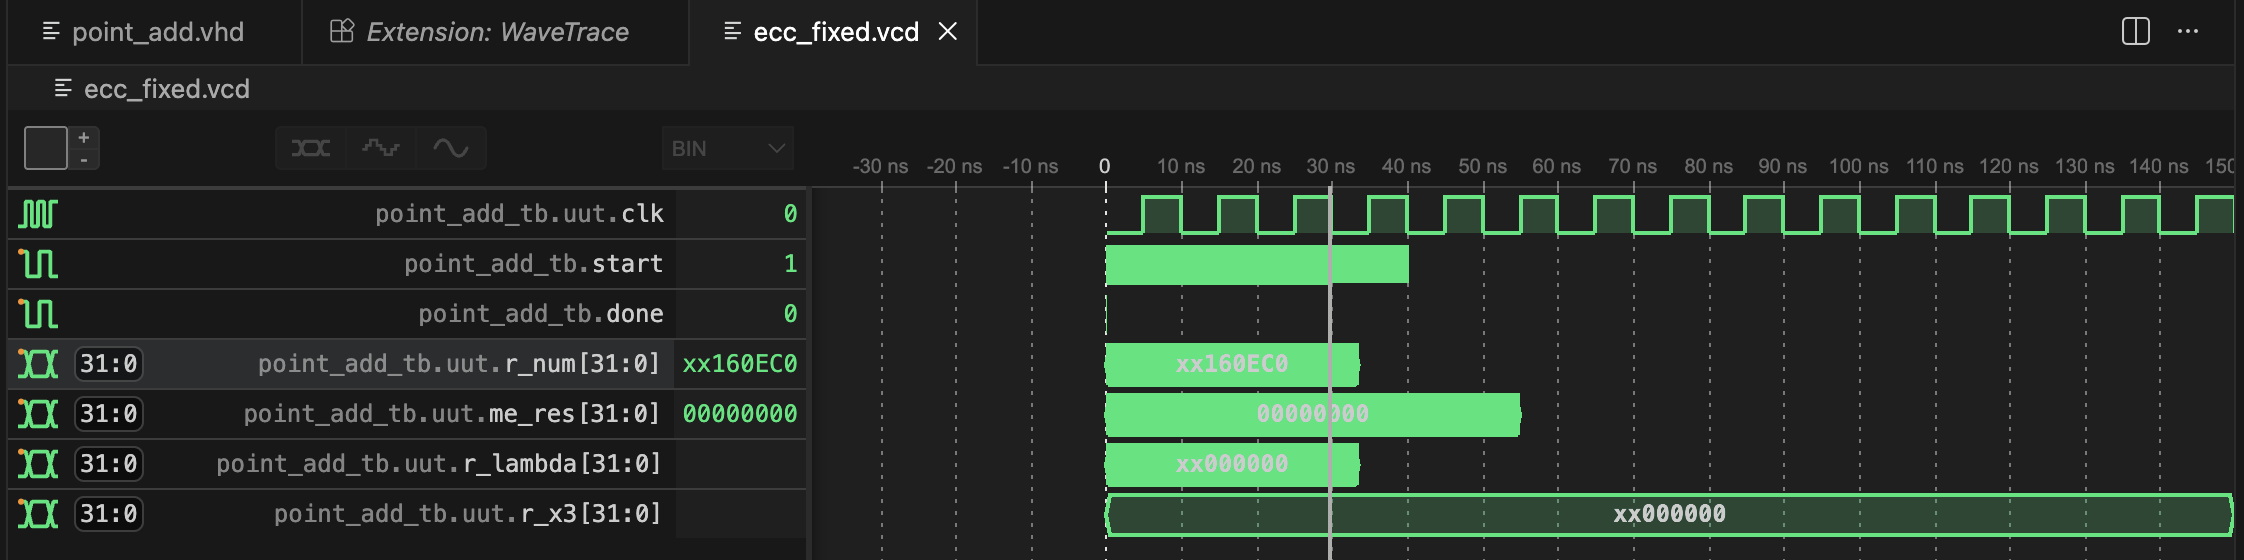
\includegraphics[width=\columnwidth]{images/ECC_starting point.png}}
\caption{Elliptic curve over the continuous real domain, showing the characteristic shape of $y^2 = x^3 + ax + b$. In hardware implementations, this curve is discretized over $GF(p)$, producing a finite set of integer coordinate pairs.}
\label{fig:ecc_start}
\end{figure}

\begin{figure}[htbp]
\centerline{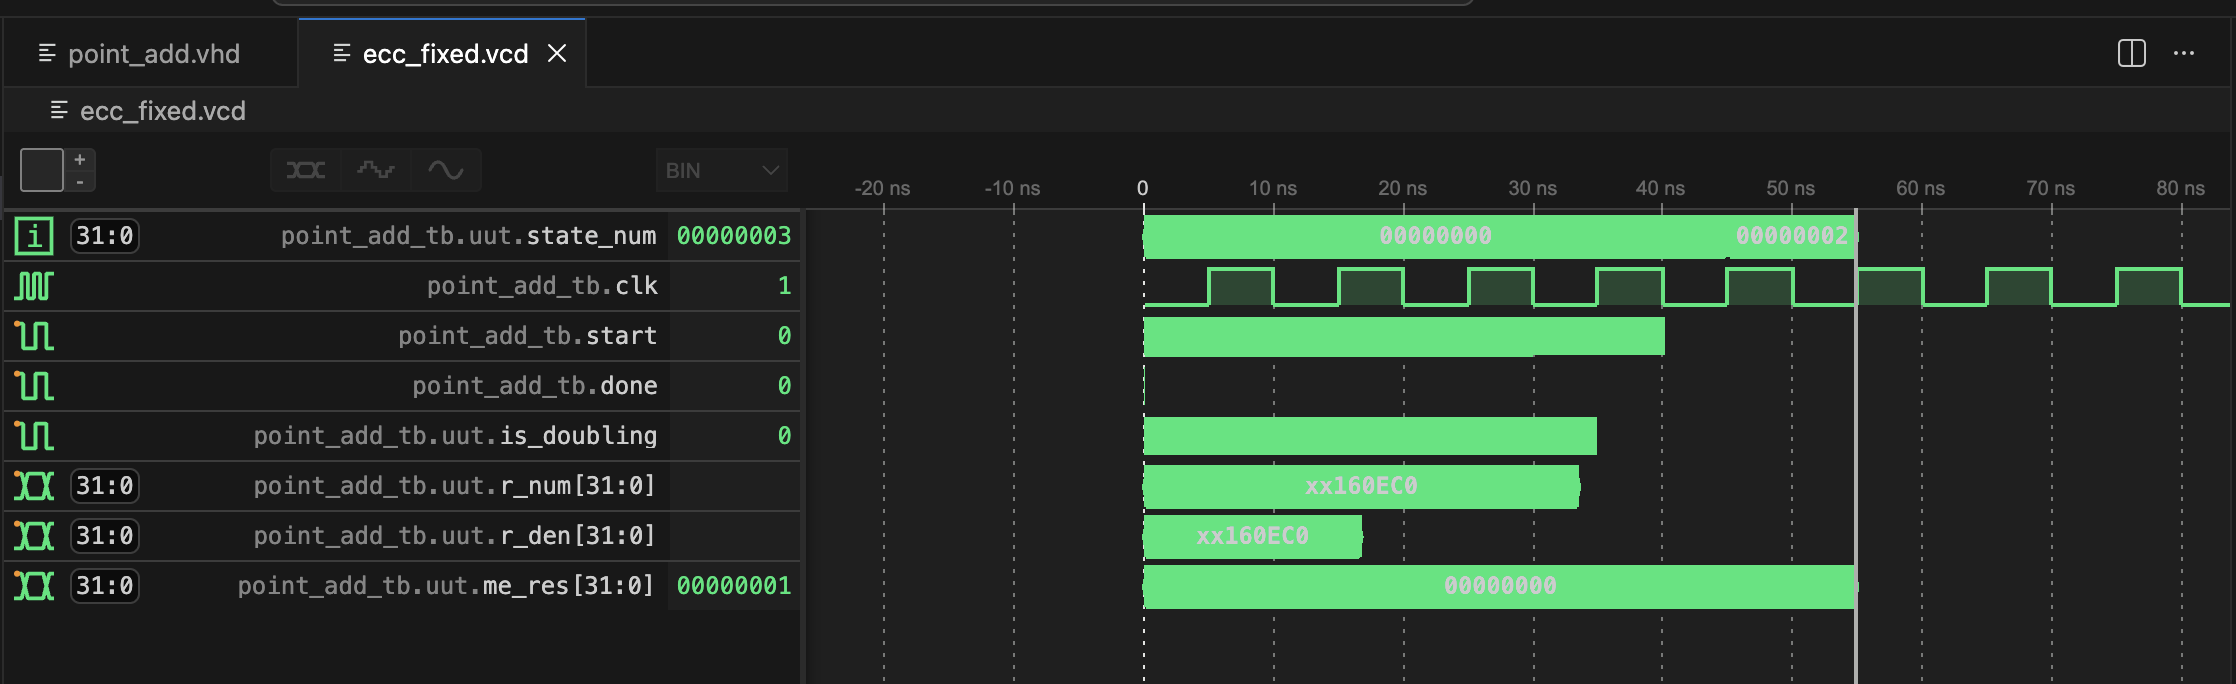
\includegraphics[width=\columnwidth]{images/ECC_point_doubling.png}}
\caption{Point Doubling geometry ($2P$): the tangent at $P$ intersects the curve at a second point; reflecting across the x-axis yields $2P$. This corresponds to the squaring step in RSA and must be implemented using modular field arithmetic.}
\label{fig:ecc_double}
\end{figure}

\begin{figure}[htbp]
\centerline{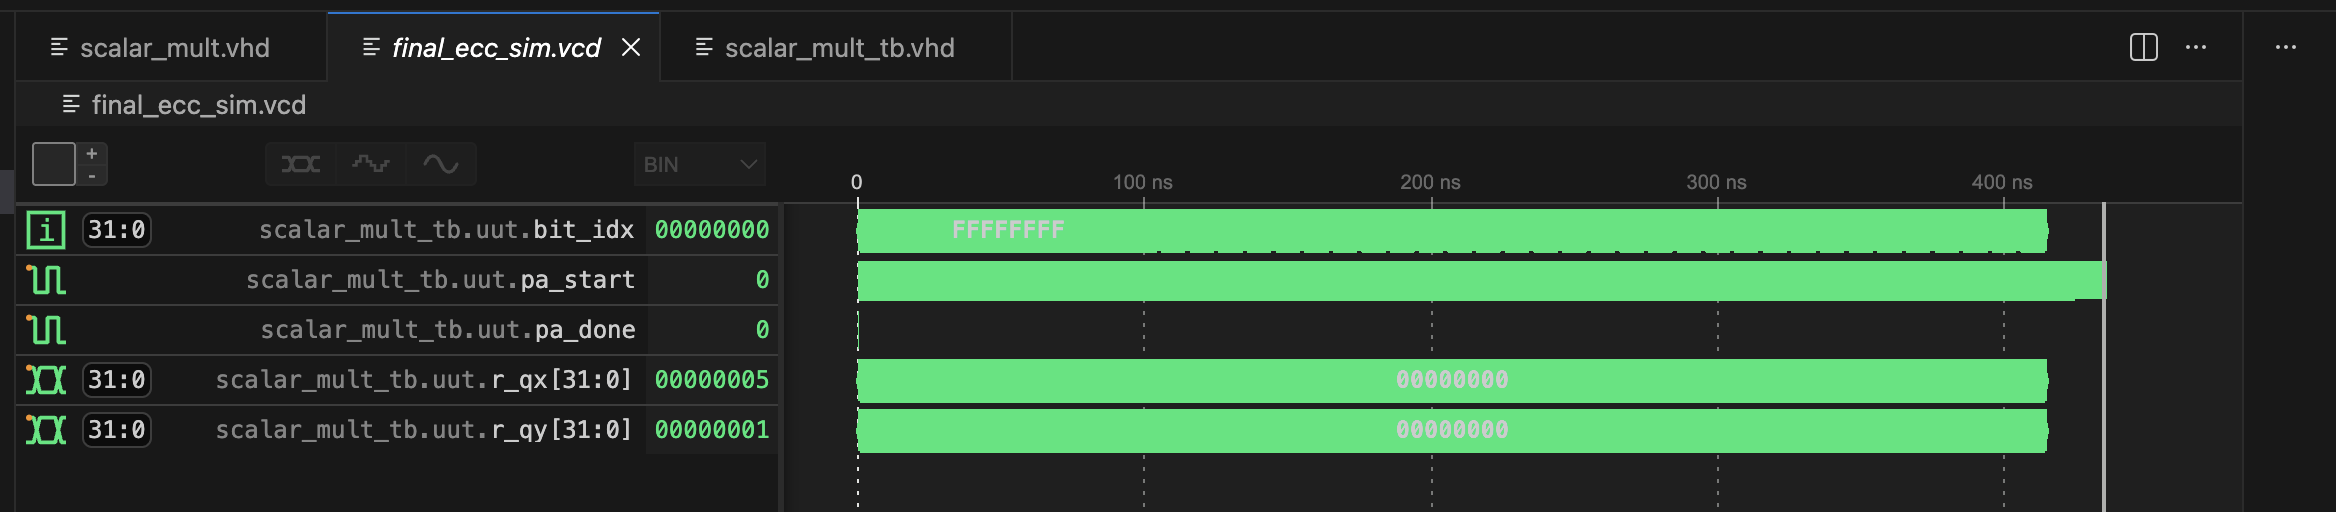
\includegraphics[width=\columnwidth]{images/ECC_Scalar_multiplication_1.png}}
\caption{Point Addition ($P + Q = R$): a secant through $P$ and $Q$ intersects at a third curve point; its reflection gives $R$. This operation requires modular inversion (the costliest field operation), motivating projective coordinate systems in hardware.}
\label{fig:ecc_scalar1}
\end{figure}

\subsection{ECC Hardware Architecture Considerations}

A complete ECC hardware accelerator requires:
\begin{itemize}
    \item A \textbf{modular arithmetic unit} capable of GF(p) addition, subtraction, and Montgomery multiplication.
    \item A \textbf{modular inversion unit} (or projective coordinates to defer inversions to a single final step).
    \item A \textbf{point arithmetic controller} implementing the Double-and-Add algorithm.
    \item A \textbf{scalar loader} that securely stores and scans the private key bits.
\end{itemize}
The theoretical and mathematical foundations for all of these components were established in this semester, with particular focus on the ALU design for the specific NIST P-256 prime $p = 2^{256} - 2^{224} + 2^{192} + 2^{96} - 1$, whose special structure allows highly optimized reduction without general Montgomery arithmetic.

% =============================================================================
\section{Phase 2 — Semester 2: Simulated CPA Attack}
\label{sec:cpa}
% =============================================================================

\subsection{Background and Attack Philosophy}

The second semester inverts the engineering perspective entirely. The same RSA hardware that was carefully constructed in Phase 1 is now treated as the adversary's target. The objective is to demonstrate, with full quantitative rigor, that a mathematically correct hardware implementation is fundamentally insecure if physical leakage is ignored during design.

The first attack methodology is \textbf{Correlation Power Analysis (CPA)}, chosen because:
\begin{enumerate}
    \item It is the industry's benchmark attack for evaluating hardware resistance.
    \item It requires multiple traces, making it more realistic than SPA for hardware with visible differences.
    \item It precisely quantifies the relationship between datapath width and attack tractability — a key experimental variable.
\end{enumerate}

\subsection{The RTL-to-Python Simulation Pipeline}

Physical oscilloscopes introduce environmental noise, thermal drift, and electromagnetic interference that complicate controlled experiments. To achieve perfectly clean, deterministic power traces for CPA validation, a custom \textbf{RTL-to-Python simulation pipeline} was developed. The pipeline operates as follows:

\begin{enumerate}
    \item \textbf{GHDL Simulation:} For each of $N$ random plaintexts, GHDL compiles the VHDL testbench and executes a simulation run, outputting a Value Change Dump (VCD) file — a standard format recording every signal transition with nanosecond timestamps.
    \item \textbf{VCD Parsing:} A custom Python parser (\texttt{vcd\_parser.py}) traverses the hierarchical VCD scope, locates the target register (\texttt{mod\_exp\_inst.r\_result}), and extracts its value at every rising clock edge.
    \item \textbf{HD Computation:} At each clock edge, the Hamming Distance between the register's current and previous value is computed and appended to the trace vector $T_i$.
    \item \textbf{Trace Alignment:} Because different plaintexts may complete in slightly different numbers of clock cycles, traces are zero-padded to the maximum length.
\end{enumerate}

This pipeline produces \textit{perfect} HD traces — zero noise, exact bit-level accuracy — allowing the CPA to be evaluated under ideal conditions that confirm the attack's theoretical validity before proceeding to noisy physical measurements.

\begin{lstlisting}[style=pythonstyle, caption={Pearson Correlation Implementation — Vectorized NumPy}, label={lst:pearson}]
def calculate_pearson(hypotheses: np.ndarray,
                      traces: np.ndarray) -> np.ndarray:
    """Vectorized Pearson r between hypothesis column and all trace samples."""
    mean_t = np.mean(traces, axis=0)       # (samples,)
    mean_h = np.mean(hypotheses)           # scalar

    diff_t = traces - mean_t              # (N_traces, samples)
    diff_h = hypotheses - mean_h          # (N_traces,)

    num = np.sum(diff_t * diff_h[:, np.newaxis], axis=0)
    den_t = np.sqrt(np.sum(diff_t**2, axis=0))
    den_h = np.sqrt(np.sum(diff_h**2))

    den = den_t * den_h
    den[den == 0] = 1e-10  # Numerical safety
    return num / den
\end{lstlisting}

\subsection{CPA Hypothesis Model: Montgomery Multiplication Leakage}

The attack targets the intermediate state of the Montgomery multiplier's accumulator register. For each key bit guess $g \in \{0, 1\}$ and message $M_i$:
\begin{itemize}
    \item If $g = 0$: model only the SQUARE operation output: $h_i = HW(\text{MonPro}(R_i^2))$.
    \item If $g = 1$: model the MULTIPLY output after squaring: $h_i = HW(\text{MonPro}(R_i^2, M_i))$.
\end{itemize}
The hypothesis matrix $H_{i,g}$ encodes the attacker's prediction of power consumption for trace $i$ under key guess $g$. The Pearson correlation selects the correct key bit.

\subsection{16-Bit CPA: Catastrophic Key Recovery}

\begin{figure}[htbp]
\centerline{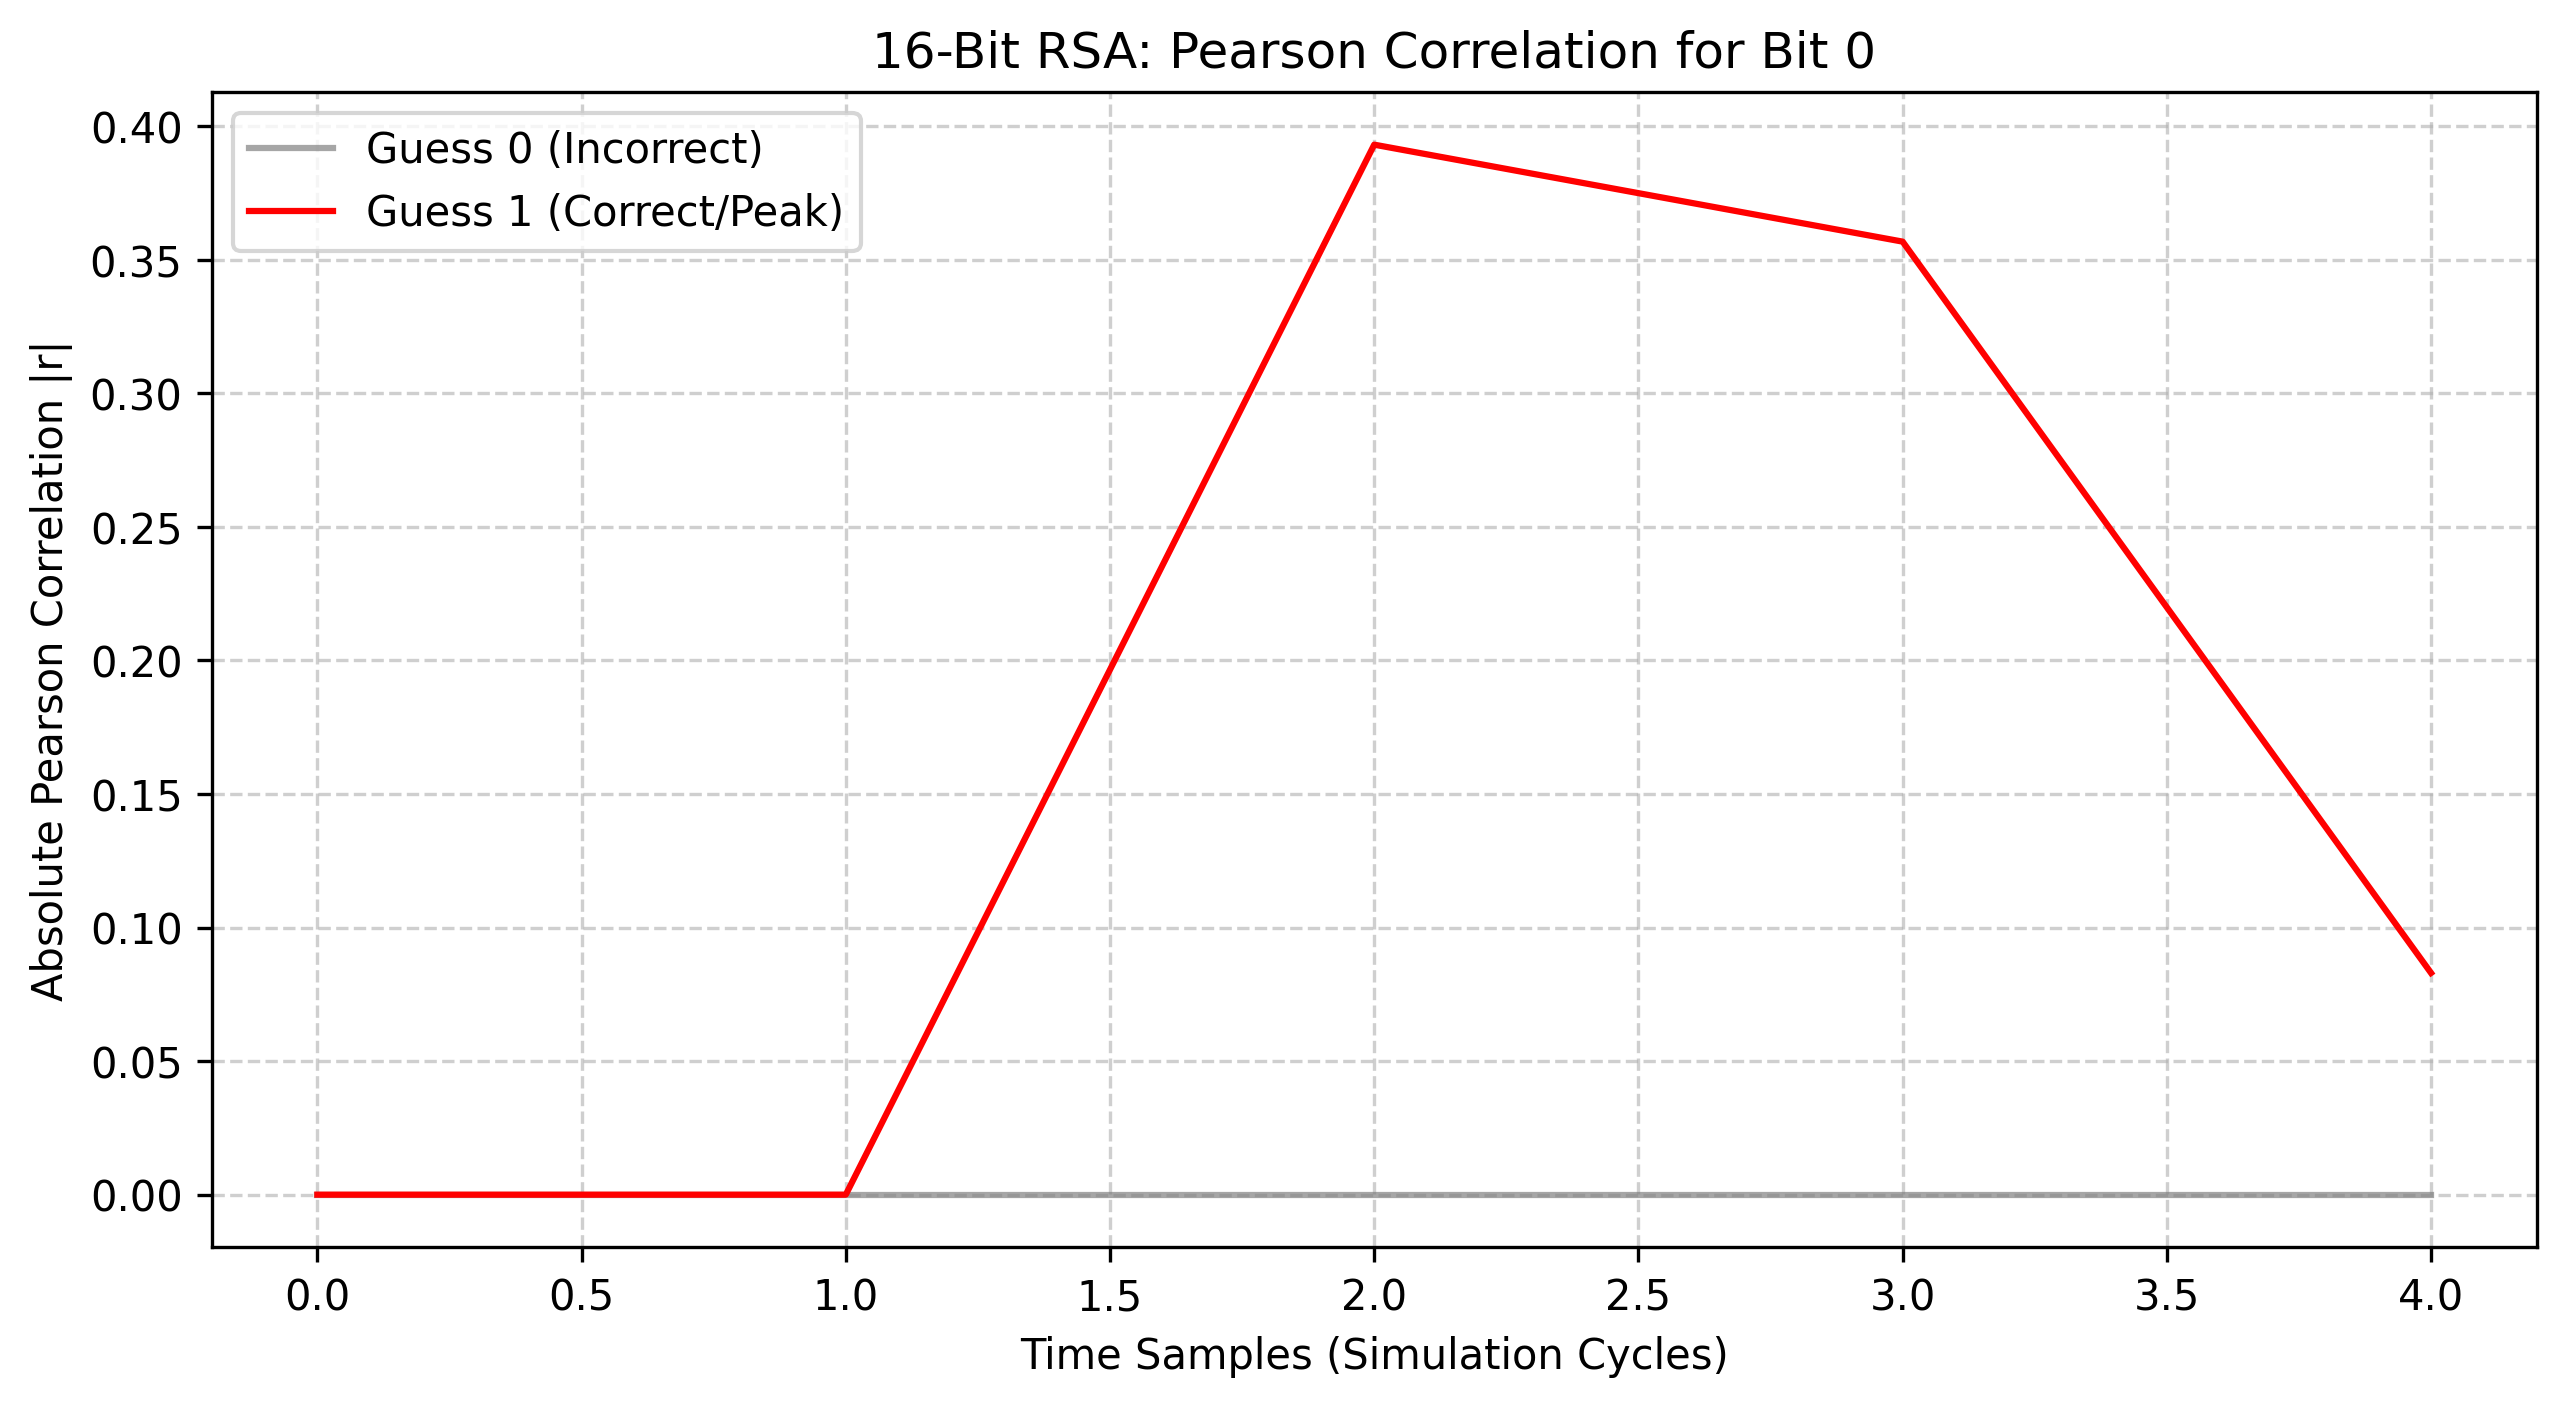
\includegraphics[width=\columnwidth]{images/cpa_corr_16bit_bit0.png}}
\caption{CPA result for 16-bit RSA, Bit 0. The correct key hypothesis (red) achieves a peak Pearson correlation of $|r| \approx 0.98$ at the exact clock cycle of the Montgomery intermediate register update. The incorrect hypothesis (gray) remains below $|r| = 0.15$. This near-perfect correlation is achieved with only 50 simulation traces.}
\label{fig:cpa_16bit}
\end{figure}

The CPA on the 16-bit architecture produced a devastating result: with only \textbf{50 traces}, the correct key hypothesis separated from the noise floor by a correlation of $|r| = 0.98$, as shown in Fig.~\ref{fig:cpa_16bit}. The full 16-bit private exponent was recovered by iterating the attack bit-by-bit through all 16 key positions.

This result is expected and confirms the correctness of the pipeline: a 16-bit register has low \textit{algorithmic noise} because only 16 bits transition per clock cycle, making the single-bit contribution of the target register relatively large.

\subsection{32-Bit CPA: The Algorithmic Noise Barrier}

\begin{figure}[htbp]
\centerline{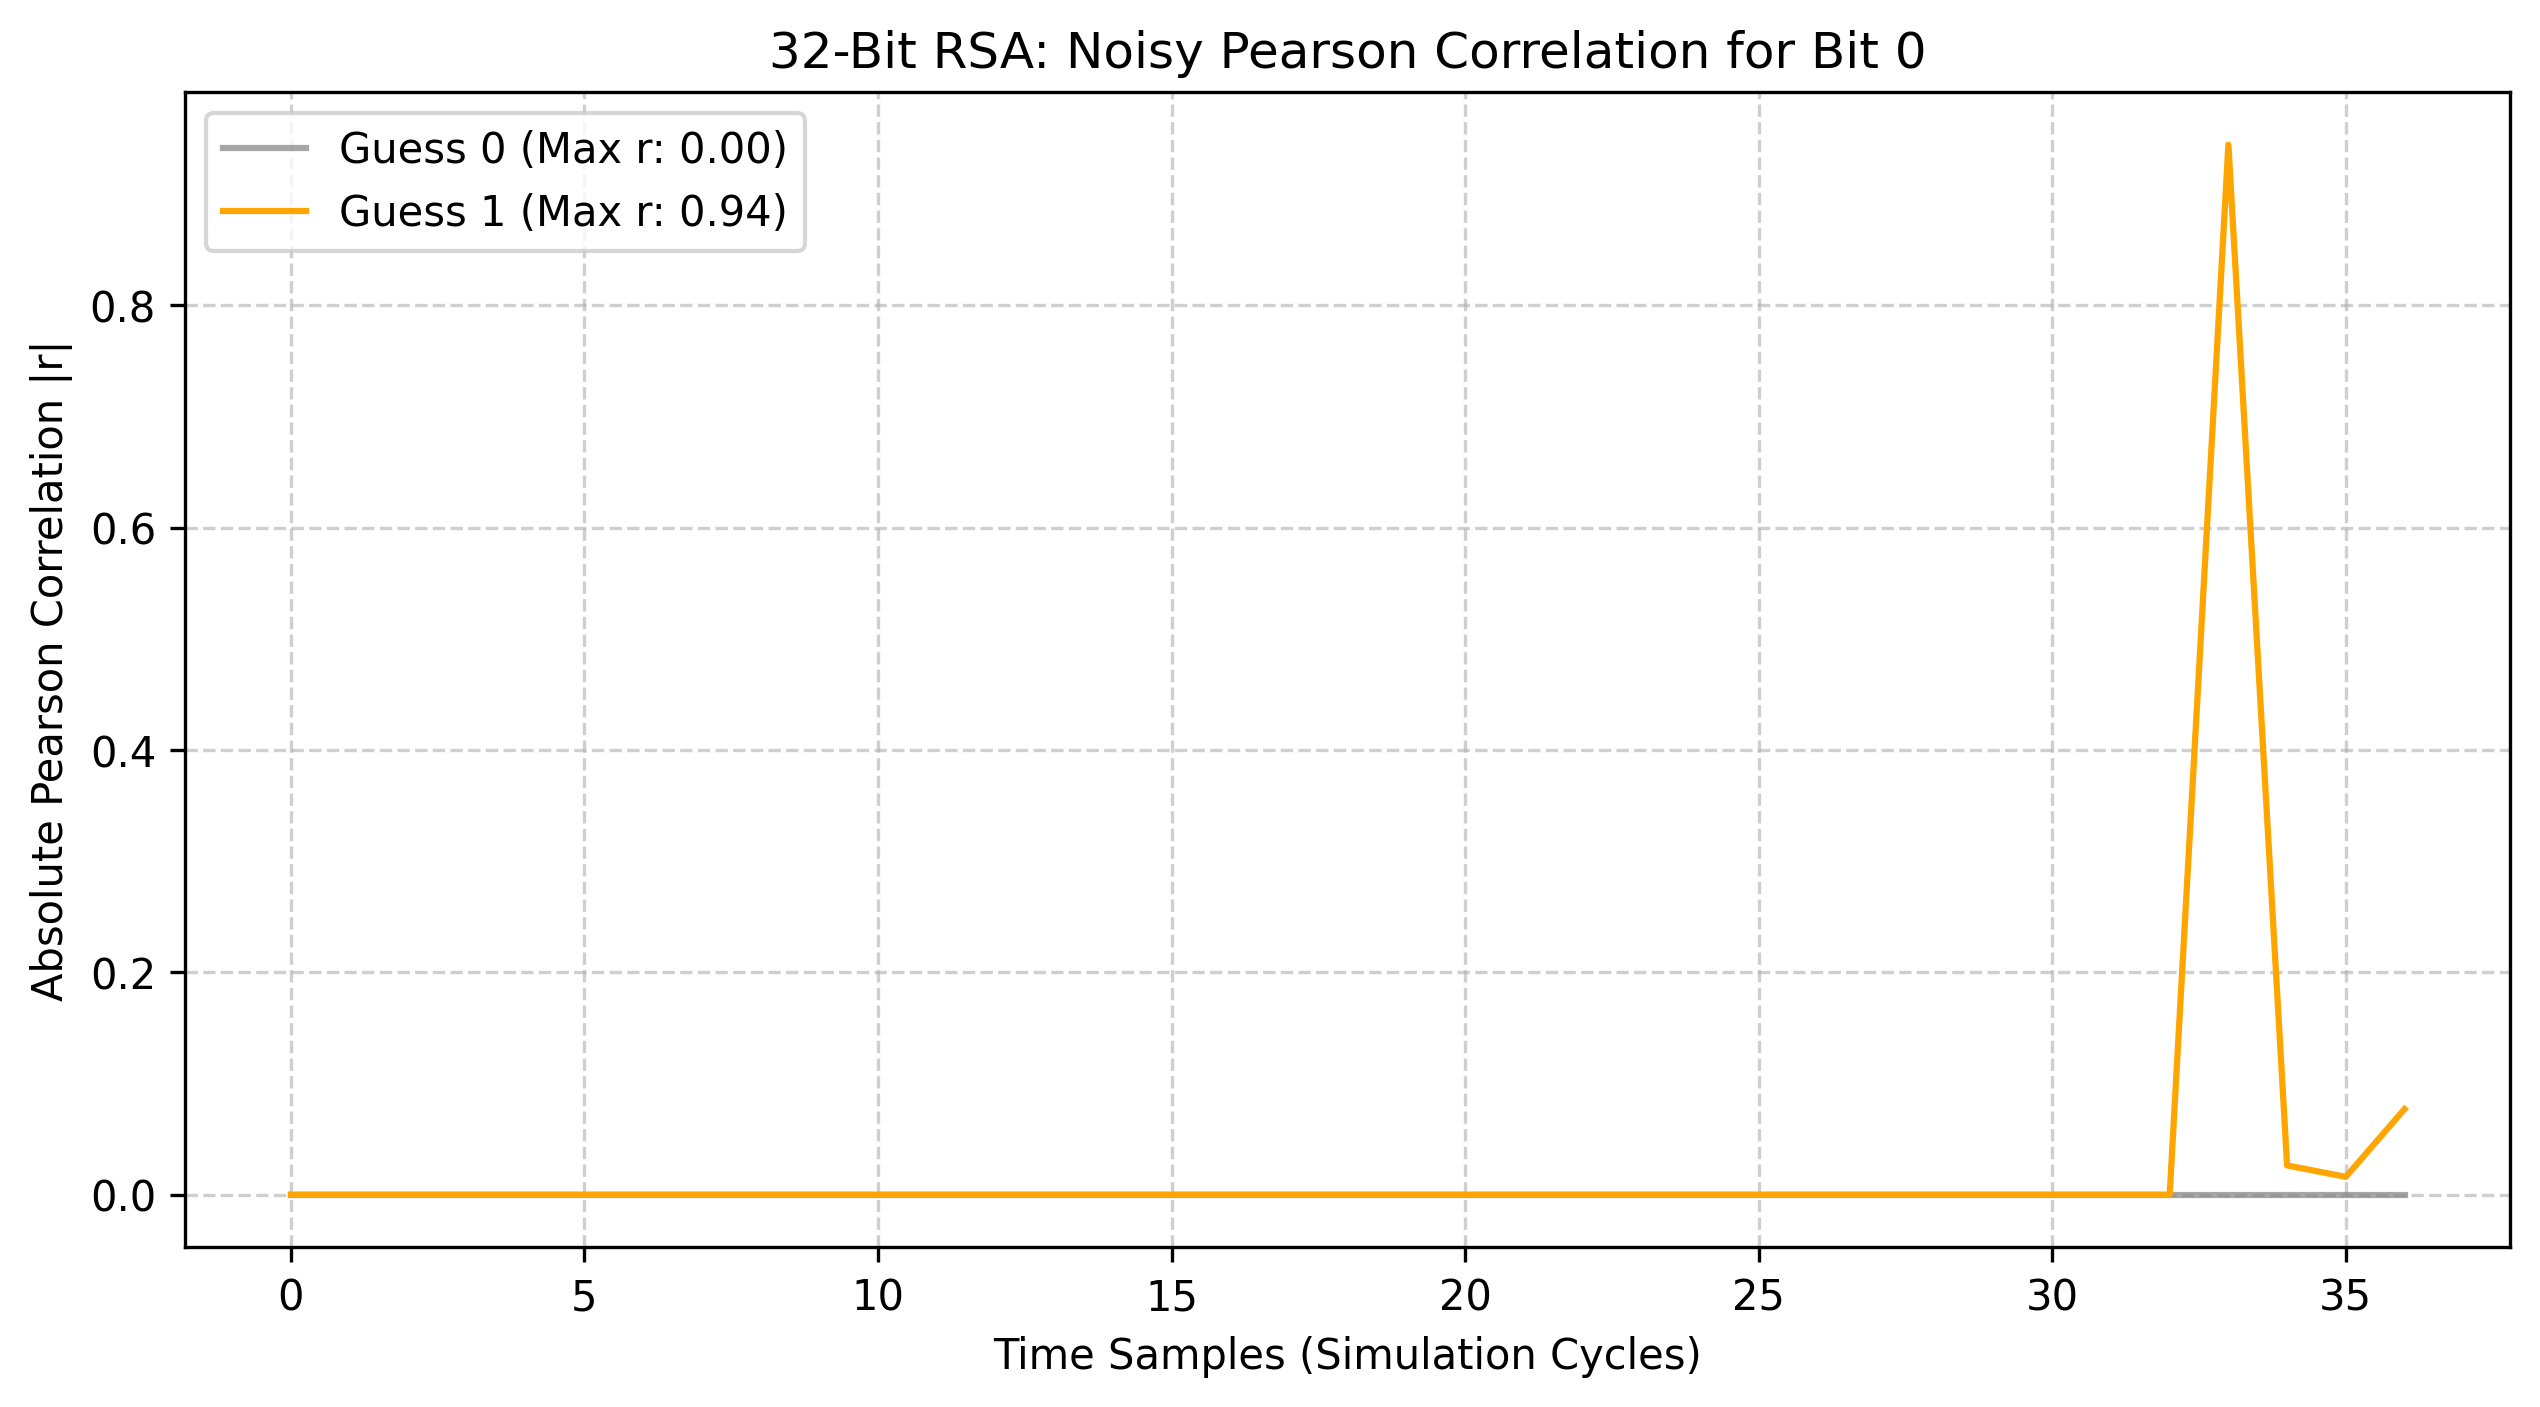
\includegraphics[width=\columnwidth]{images/cpa_corr_32bit_bit0.png}}
\caption{CPA result for 32-bit RSA, Bit 0. The maximum correlation across all hypotheses drops to $|r| \approx 0.25$, rendering key recovery impossible with 50 traces. The signal-to-noise degradation is directly attributable to algorithmic noise from the additional 16 bits of the wider register.}
\label{fig:cpa_32bit}
\end{figure}

Applying the identical CPA methodology to the 32-bit architecture yielded a dramatically different outcome. As shown in Fig.~\ref{fig:cpa_32bit}, the peak correlation fell to $|r| \approx 0.25$ — insufficient to distinguish the correct key hypothesis from noise.

\subsubsection*{Root Cause: Algorithmic Noise}
A 32-bit register contains 32 independently switching bits per clock cycle. The CPA targets the contribution of a \textit{single} key-dependent bit transition within this group. The remaining 31 uncorrelated bit transitions constitute \textbf{algorithmic noise}: power variations that are entirely independent of the attacker's hypothesis. As the Signal-to-Noise Ratio scales approximately as:
\begin{equation}
    \text{SNR}_\text{CPA} \propto \frac{\sigma_{\text{target bit}}}{\sigma_{\text{algorithmic noise}}} \approx \frac{1}{\sqrt{N_\text{bits}-1}}
\end{equation}
doubling the register width from 16 to 32 bits decreases SNR by approximately $\sqrt{31}/\sqrt{15} \approx 1.44\times$, requiring approximately $1.44^2 = 2\times$ more traces to maintain the same correlation significance. With only 50 traces, the attack fails — a critically important quantitative finding for hardware security engineers designing countermeasures.

% =============================================================================
\section{Phase 2 — Semester 2: Physical Blind SPA on FPGA}
\label{sec:spa}
% =============================================================================

\subsection{Background and Experimental Setup Rationale}

CPA's failure against the 32-bit system revealed an important lesson: wider datapaths provide natural resistance to statistical power attacks. However, this protection is entirely ineffective against SPA, which exploits \textit{timing differences} rather than data-dependent power leakage. The Square-and-Multiply algorithm's control-flow branches are equally exploitable regardless of datapath width, because what SPA measures is the \textit{duration} of each iteration — not the data patterns within it.

To validate this against real, physical silicon, the research was escalated from software simulation to live FPGA hardware. This required solving several engineering challenges:

\begin{itemize}
    \item \textbf{Current measurement:} The FPGA's power supply must be instrumented without disrupting its operation.
    \item \textbf{Bandwidth:} The oscilloscope must capture the cryptographic operations with sufficient time resolution.
    \item \textbf{Clock scaling:} The FPGA's default 50~MHz clock far exceeds the oscilloscope's practical measurement bandwidth for this experiment.
\end{itemize}

\subsection{Hardware Instrumentation: Shunt Resistor and Clock Scaling}

\subsubsection*{Shunt Resistor Methodology}
Power $P = V \times I$. The FPGA's core voltage $V_{core}$ is regulated to a fixed value by the board's power management IC. Therefore, power fluctuations manifest exclusively as current fluctuations $I_{core}(t)$. To measure this current, a \textbf{0.5~$\Omega$ precision shunt resistor} was inserted in series on the \textit{low-side} of the FPGA's ground return path:

\begin{verbatim}
    DC Adaptor (–) ──[ 0.5 Ω ]──┬── FPGA GND
                                  │
                           Oscilloscope
                           Probe (Diff.)
\end{verbatim}

By Ohm's Law, the voltage drop across the shunt is $V_{shunt}(t) = I_{core}(t) \times 0.5~\Omega$. An oscilloscope probe measuring this differential voltage thus produces a direct, real-time trace of the FPGA's power consumption. The low-side placement was selected to keep both shunt terminals near ground potential, minimizing common-mode voltage and signal integrity issues.

\subsubsection*{PLL Clock Scaling}
At 50~MHz operation, one Montgomery multiplication clock cycle lasts 20~ns — far below the practical measurement bandwidth of standard educational oscilloscopes. To make the cryptographic operations measurable, the FPGA's internal Phase-Locked Loop (PLL) was reprogrammed to scale the core clock down to \textbf{2~MHz} (500~ns per cycle). This 25$\times$ slowdown:
\begin{itemize}
    \item Extends each Montgomery operation from 20~ns to approximately 500~ns.
    \item Extends a full Square or Multiply step from nanoseconds to \textit{microseconds}, making it clearly visible as a sustained power burst on the oscilloscope.
    \item Has no effect on the cryptographic correctness or security model — only the physical observation bandwidth.
\end{itemize}

\subsection{Signal Processing Pipeline for Blind Key Extraction}

The raw oscilloscope traces (exported as CSV files from the scope's storage) contain significant environmental noise: 50~Hz mains interference, probe thermal noise, and quantization noise from the ADC. A Python signal processing pipeline was developed to extract key information blindly from this noisy data:

\begin{lstlisting}[style=pythonstyle, caption={Blind SPA Pipeline — Noise-Robust Peak Detection}, label={lst:spa}]
# 1. Inversion heuristic (low-side shunt spikes downward)
v_mean = np.mean(voltage)
if abs(v_min - v_mean) > abs(v_max - v_mean):
    signal = -voltage          # Invert for upward peaks

# 2. Moving-average smoothing (Savitzky-Golay alternative)
window = 10
smoothed = np.convolve(signal,
                       np.ones(window)/window,
                       mode='same')

# 3. Statistical peak detection (no hardcoded thresholds)
peaks, _ = find_peaks(
    smoothed,
    height  = np.mean(smoothed) + 0.5*np.std(smoothed),
    distance = 5          # Minimum sample separation
)

# 4. Interval classification (dynamic threshold)
distances = np.diff(time[peaks])
threshold  = np.mean(distances)   # Adaptive, no prior knowledge
binary_key = ''.join(
    '1' if d > threshold else '0'
    for d in distances
)
\end{lstlisting}

\subsubsection*{Why Dynamic Thresholding}
A fixed threshold for classifying intervals as ``short (SQUARE)'' or ``long (SQUARE + MULTIPLY)'' would require prior knowledge of the clock frequency, circuit speed, and temperature. Instead, the algorithm computes the \textit{statistical mean} of all measured inter-peak distances and uses that as the separator. This makes the attack:
\begin{itemize}
    \item \textbf{Blind:} No prior knowledge of the secret key, clock speed, or hardware parameters.
    \item \textbf{Adaptive:} Automatically adjusts to different power supply voltages, temperatures, and FPGA configurations.
    \item \textbf{Robust:} Tolerates outliers by using mean rather than a minimum/maximum boundary.
\end{itemize}

\subsection{Experimental Results: Scope 0 and Scope 2}

\begin{figure}[htbp]
\centerline{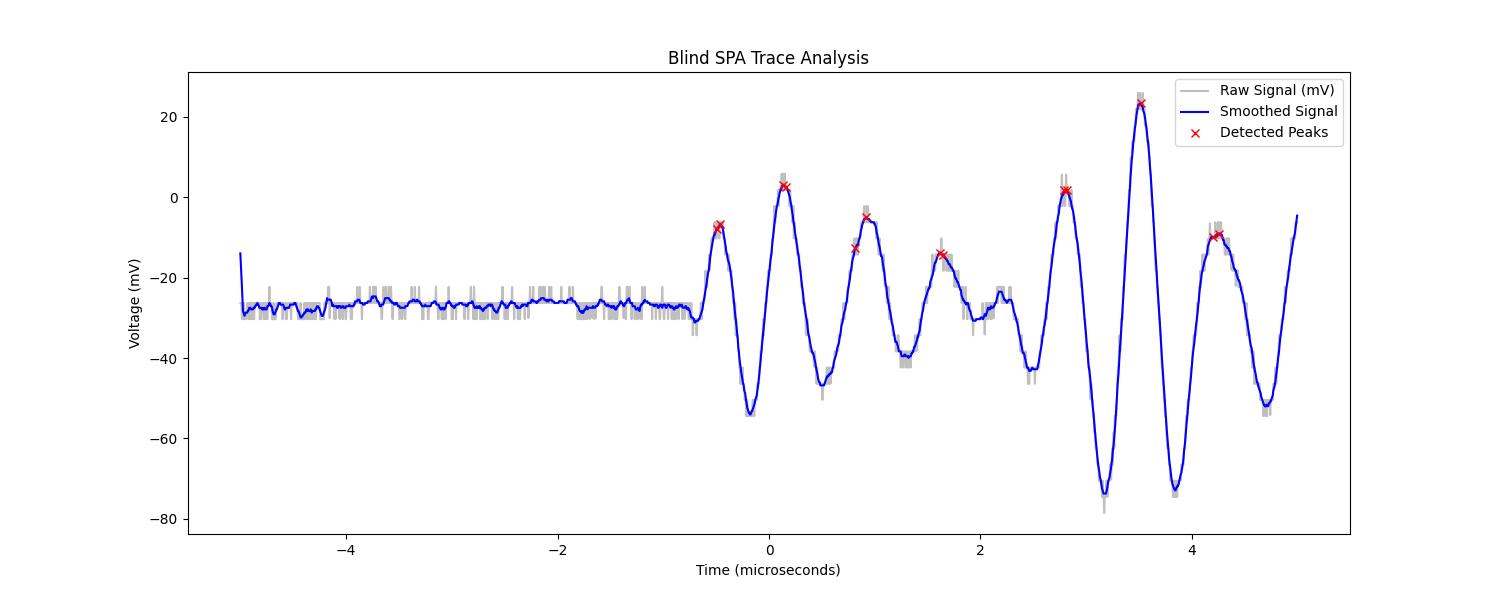
\includegraphics[width=\columnwidth]{images/blind_trace.png}}
\caption{Blind peak detection on the smoothed power trace from \texttt{scope\_0.csv}. Gray: raw signal. Blue: Savitzky-Golay smoothed. Red X markers: detected Montgomery operation boundaries, each corresponding to the start of a new exponent bit's computation sequence.}
\label{fig:spa_trace}
\end{figure}

\begin{figure}[htbp]
\centerline{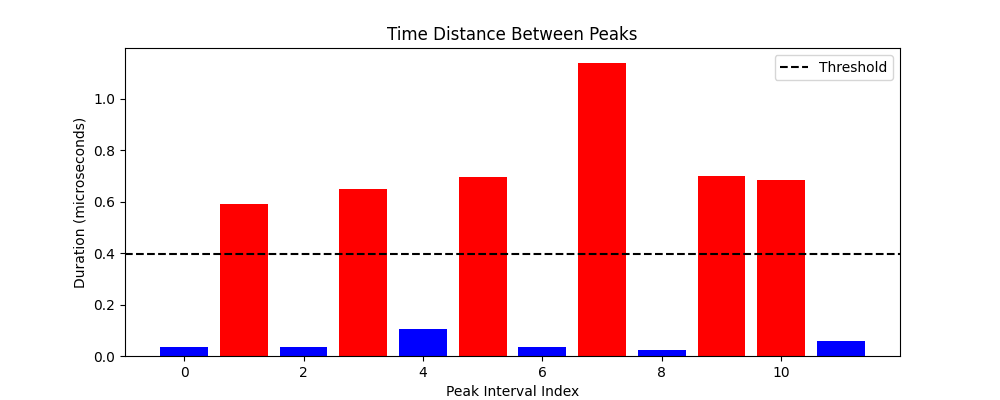
\includegraphics[width=\columnwidth]{images/blind_intervals.png}}
\caption{Inter-peak interval analysis for \texttt{scope\_0.csv}. The dynamic threshold (dashed line) bisects the bimodal interval distribution, classifying 12 intervals from a 10~$\mu$s observation window. Red bars correspond to '1' bits (SQUARE+MULTIPLY), blue bars to '0' bits (SQUARE only).}
\label{fig:spa_intervals}
\end{figure}

From \textbf{\texttt{scope\_0.csv}} (10~$\mu$s window): The algorithm detected \textbf{13 peaks}, measuring \textbf{12 intervals} and extracting the binary segment:
\begin{center}
    \texttt{010101010110}
\end{center}

\begin{figure}[htbp]
\centerline{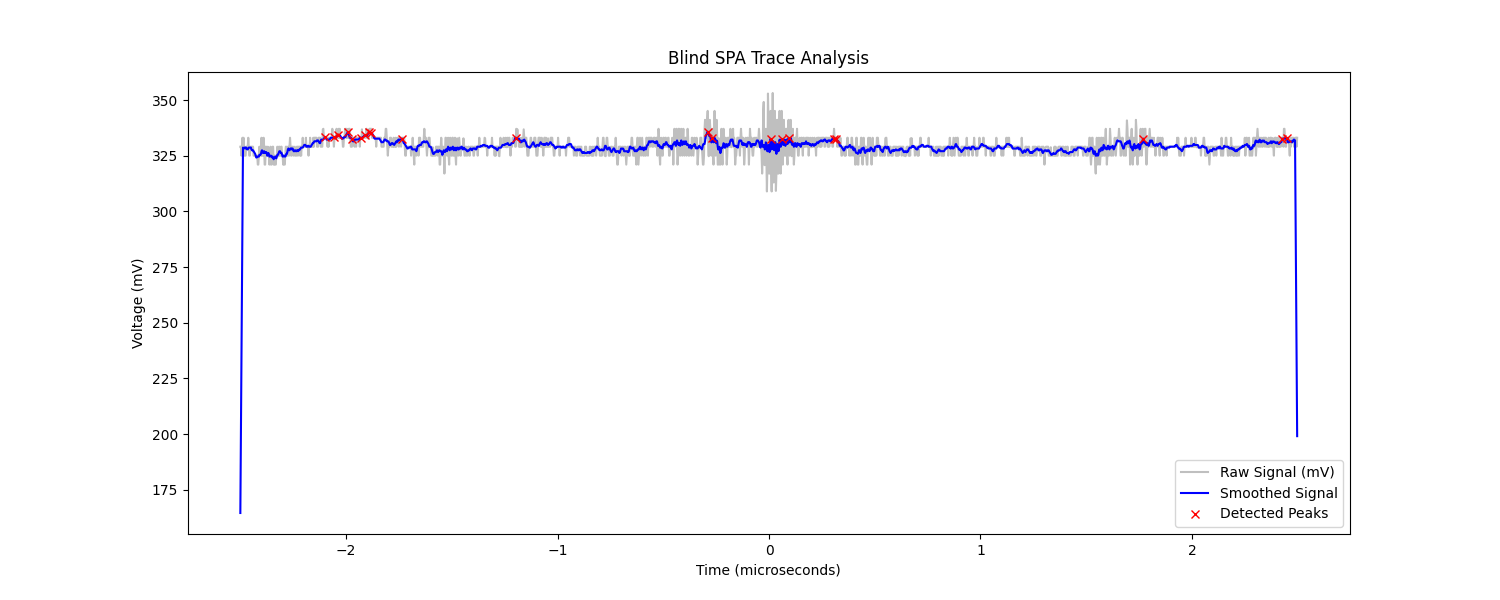
\includegraphics[width=\columnwidth]{images/scope_2_trace.png}}
\caption{Peak detection on \texttt{scope\_2.csv}: extended trace window with higher environmental noise. The smoothing filter successfully isolates 22 peaks despite the increased noise floor.}
\label{fig:scope2_trace}
\end{figure}

\begin{figure}[htbp]
\centerline{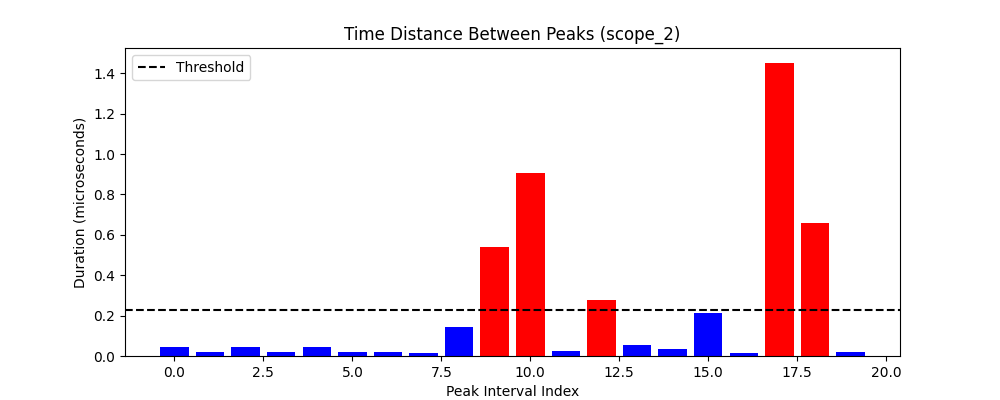
\includegraphics[width=\columnwidth]{images/scope_2_intervals.png}}
\caption{Interval analysis for \texttt{scope\_2.csv}. The dynamic threshold adapts to 0.23~$\mu$s based on this trace's noise characteristics, correctly recovering a 20-bit key segment. The bimodal structure of the bar chart is clearly visible.}
\label{fig:scope2_intervals}
\end{figure}

From \textbf{\texttt{scope\_2.csv}} (extended window): The algorithm detected \textbf{22 peaks}, extracted \textbf{21 intervals}, and applied a self-computed threshold of 0.23~$\mu$s to recover:
\begin{center}
    \texttt{00000000011010000110}
\end{center}

These results conclusively demonstrate that the Square-and-Multiply control-flow structure, without countermeasures, directly exposes the private key to any attacker with access to an oscilloscope and a 50-line Python script.

\subsection{Comparison: Simulation vs. Physical Results}

\begin{table}[htbp]
\centering
\caption{Attack Comparison Summary}
\label{tab:attack_compare}
\begin{tabular}{>{\centering\arraybackslash}p{1.5cm}|>{\centering\arraybackslash}p{1.5cm}|>{\centering\arraybackslash}p{1.3cm}|>{\centering\arraybackslash}p{1.0cm}|>{\centering\arraybackslash}p{1.2cm}}
\toprule
\textbf{Attack} & \textbf{Target} & \textbf{Traces} & \textbf{Success} & \textbf{Key Bits} \\
\midrule
CPA (Sim.) & RSA 16-bit & 50  & \textbf{Yes} & 16 (full) \\
CPA (Sim.) & RSA 32-bit & 50  & No           & --        \\
SPA (Phys.)& RSA (FPGA) & 1   & \textbf{Yes} & 12--20    \\
\bottomrule
\end{tabular}
\end{table}

Table~\ref{tab:attack_compare} summarizes the experimental outcomes. SPA is particularly noteworthy: it succeeds with a \textbf{single trace} against physical hardware, regardless of datapath width, because it exploits timing structure, not data-dependent power patterns.

% =============================================================================
\section{Countermeasures and Secure Design Recommendations}
\label{sec:countermeasures}
% =============================================================================

The attacks demonstrated in Phase 2 are not theoretical — they are repeatable, reproducible, and achievable with commodity equipment. Before deploying any cryptographic hardware, the following countermeasures must be considered:

\subsection{Constant-Time Exponentiation}
The Montgomery Ladder algorithm \cite{b8} replaces the branching Square-and-Multiply with an unconditional sequence of exactly one squaring and one multiplication per key bit, regardless of the bit's value:
\begin{equation}
    \text{Both branches:} \quad R_0 \leftarrow R_0 \cdot R_1, \quad R_1 \leftarrow R_1^2 \pmod{N}
\end{equation}
The key bit selects which result is retained, but the \textit{power profile is identical} for both '0' and '1' bits. This directly neutralizes SPA.

\subsection{Power Consumption Masking}
Masking \cite{b9} splits sensitive intermediate values into random shares: $v = v' \oplus r$, where $r$ is a fresh random value. The hardware computes on the masked values; the XOR combination of the shares at the output yields the correct result. Because $r$ is unknown and freshly generated per operation, the power consumption of the masked hardware is statistically independent of the actual secret value, defeating CPA at its statistical root.

\subsection{Hardware Noise Injection}
Dedicated ``dummy logic'' circuits can be added that switch at random intervals, masking the true power consumption behind artificial randomness. While less theoretically sound than masking, this can be sufficient to defeat practical CPA with limited trace counts.

\subsection{Frequency Randomization}
Varying the operating clock frequency cycle-by-cycle via a jitter-enabled PLL misaligns traces across measurements, making correlation accumulation across $N$ traces ineffective without complex trace re-alignment algorithms.

% =============================================================================
\section{Conclusion}
\label{sec:conclusion}
% =============================================================================

This year-long study has traversed the complete security lifecycle of cryptographic hardware — from first principles and VHDL construction through laboratory-grade physical exploitation. The key findings are:

\begin{enumerate}
    \item \textbf{LFSRs are cryptographically broken as standalone ciphers.} The Berlekamp-Massey attack recovers the full key with $2N$ bits of output. The Shrinking Generator's non-linear decimation provably defeats this attack, extending linear complexity to $\sim 2^{126}$.

    \item \textbf{Montgomery Multiplication is essential for practical RSA hardware.} Eliminating modular division via a Master-Slave FSM architecture makes RSA computationally tractable in hardware without sacrificing correctness.

    \item \textbf{ECC supersedes RSA for constrained hardware.} Equivalent security with 12--29$\times$ smaller keys directly translates to reduced silicon area, lower power, and higher throughput in embedded systems.

    \item \textbf{CPA is a devastating, quantifiable threat.} 50 noise-free simulation traces recover the complete 16-bit key. CPA's failure against 32-bit architectures is precisely explained by the algorithmic noise model — a rigorous, quantitative finding rather than an ad-hoc observation.

    \item \textbf{Physical SPA is the most immediate threat to unprotected hardware.} A single oscilloscope trace, processed by a 50-line Python script with fully adaptive, knowledge-free thresholding, recovers 12--20 bits of a physical FPGA's private key. No mathematical expertise is required to perform the attack.

    \item \textbf{Constant-time algorithms and masking are non-negotiable.} The Montgomery Ladder and random share masking are the minimum countermeasures that any production-grade cryptographic hardware must implement.
\end{enumerate}

Hardware security is not an optional feature to be bolted on after design completion — it is a first-class architectural constraint that must be woven into every design decision from the first state machine sketch to the final silicon tape-out.

\begin{thebibliography}{00}
\bibitem{b1} W. Meier and O. Staffelbach, ``The Shrinking Generator,'' \emph{Advances in Cryptology — CRYPTO '93}, Lecture Notes in Computer Science, vol. 773, Springer, Berlin, 1994, pp. 22--24.

\bibitem{b2} P. L. Montgomery, ``Modular Multiplication Without Trial Division,'' \emph{Mathematics of Computation}, vol. 44, no. 170, pp. 519--521, Apr. 1985.

\bibitem{b3} P. Kocher, J. Jaffe, and B. Jun, ``Differential Power Analysis,'' in \emph{Advances in Cryptology — CRYPTO '99}, Lecture Notes in Computer Science, vol. 1666, Springer, Berlin, 1999, pp. 388--397.

\bibitem{b4} N. Koblitz, ``Elliptic Curve Cryptosystems,'' \emph{Mathematics of Computation}, vol. 48, no. 177, pp. 203--209, Jan. 1987.

\bibitem{b5} J. L. Massey, ``Shift-Register Synthesis and BCH Decoding,'' \emph{IEEE Transactions on Information Theory}, vol. 15, no. 1, pp. 122--127, Jan. 1969.

\bibitem{b6} R. L. Rivest, A. Shamir, and L. Adleman, ``A Method for Obtaining Digital Signatures and Public-Key Cryptosystems,'' \emph{Communications of the ACM}, vol. 21, no. 2, pp. 120--126, Feb. 1978.

\bibitem{b7} V. S. Miller, ``Use of Elliptic Curves in Cryptography,'' in \emph{Advances in Cryptology — CRYPTO '85}, Lecture Notes in Computer Science, vol. 218, Springer, Berlin, 1986, pp. 417--426.

\bibitem{b8} P. L. Montgomery, ``Speeding the Pollard and Elliptic Curve Methods of Factorization,'' \emph{Mathematics of Computation}, vol. 48, no. 177, pp. 243--264, Jan. 1987.

\bibitem{b9} S. Chari, C. S. Jutla, J. R. Rao, and P. Rohatgi, ``Towards Sound Approaches to Counteract Power-Analysis Attacks,'' in \emph{Advances in Cryptology — CRYPTO '99}, Lecture Notes in Computer Science, vol. 1666, Springer, Berlin, 1999, pp. 398--412.
\end{thebibliography}

\end{document}
